\documentclass[12pt,final]{report}
%\documentclass[11pt,letterpaper,twoside,openright]{book}

\usepackage{fullpage}
\usepackage{graphicx}
\usepackage{setspace}
%\usepackage{amsthm}
%\usepackage{multirow}
\usepackage{algorithm2e}
\usepackage{algorithmic}
%\usepackage{algorithm}
\usepackage{amsmath}
\usepackage{amssymb}
%\usepackage{float}
\usepackage{url}
%\usepackage{amsmath}
%\usepackage{amsfonts}
%\usepackage{flafter}
%\usepackage{natbib}
%\usepackage{epstopdf}
%\usepackage{colortbl}
\usepackage{subfigure}
\usepackage[]{hyperref}
\hypersetup{
    pdftitle={Leveraging Workload Relocation and Resource Pruning for Electricity Cost Minimization in Service Provider Networks},
    pdfauthor={Muhammad Saqib Ilyas},
    pdfsubject={Computer Networks},
    pdfkeywords={Energy Efficiency, Electricity Cost},
    bookmarksnumbered=true,     
    bookmarksopen=true,         
    bookmarksopenlevel=1,       
    colorlinks=true,            
    pdfstartview=Fit,           
    pdfpagemode=UseOutlines,    % this is the option you were lookin for
    pdfpagelayout=TwoPageRight
}
%\usepackage{latex8}
%\usepackage{times}
    
\renewcommand{\th}{\textsuperscript{th}}
\newcommand{\nd}{\textsuperscript{nd}}
\newcommand{\st}{\textsuperscript{st}}
\newcommand{\rd}{\textsuperscript{rd}}
\newcommand{\sq}{\textsuperscript{2}}

%\singlespacing
\doublespacing

\begin{document}
    
%%%%%%%%%%%%%%%%%%%%%%%%%%%%%%%%%%%%%%%%%%%%%%%%%%%%%%%%%%%%%%%%%%%%%%%%%%%
%%%%%%%%%%%%%%%%           The title page           %%%%%%%%%%%%%%%%%%%%%%%
%%%%%%%%%%%%%%%%%%%%%%%%%%%%%%%%%%%%%%%%%%%%%%%%%%%%%%%%%%%%%%%%%%%%%%%%%%%
\newpage
\thispagestyle{empty}
\begin{center}
  \vspace*{0.2in}
  {\LARGE \bf Leveraging Workload Relocation and Resource Pruning for Electricity Cost Minimization in Service Provider Networks}\\
  \vspace*{0.5in}
  {\Large \bf PhD Thesis}\\

  \vspace*{0.4in}
  {\Large\bf Muhammad Saqib Ilyas}\\
    \vspace*{0.2in}
  {\Large 2005-06-0024}\\
  \vspace*{0.4in}
  {\Large\bf Advisor: Zartash Afzal Uzmi}\\

	\vspace*{0.4in}
  \begin{center}
   
\includegraphics[scale = 0.5]{./pics/lums.eps}
  \end{center}
  \vspace*{0.4in}  
  {\Large\bf Department of Computer Science} \\
  \vspace*{0.2in}
  {\Large\bf Syed Babar Ali School of Science and Engineering} \\
  \vspace*{0.2in}
  {\Large \bf Lahore University of Management Sciences}
  
  
\end{center}
%%%%%%%%%%%%%%%%%%%%%%%%%%%%%%%%%%%%%%%%%%%%%%%%%%%%%%%%%%%%%%%%%%%%%%%%%%%
%%%%%%%%%%%%%%%% The dedication page, of you have one  %%%%%%%%%%%%%%%%%%%%
%%%%%%%%%%%%%%%%%%%%%%%%%%%%%%%%%%%%%%%%%%%%%%%%%%%%%%%%%%%%%%%%%%%%%%%%%%%
\newpage
\thispagestyle{empty}
\begin{center}
 \vspace*{3in}
  \textit{\LARGE {Dedicated to dedication}}\\

\end{center}

%%%%%%%%%%%%%%%%%%%%%%%%%%%%%%%%%%%%%%%%%%%%%%%%%%%%%%%%%%%%%%%%%%%%%%%%%%%
%%%%%%%%    Signature Page   Here                                 %%%%%%%%%
%%%%%%%%%%%%%%%%%%%%%%%%%%%%%%%%%%%%%%%%%%%%%%%%%%%%%%%%%%%%%%%%%%%%%%%%%%%
\newpage
\thispagestyle{empty}
\begin{center}
  \vspace*{1cm}
\textbf{\Large Lahore University of Management Sciences}\\
\vspace*{1cm} \textbf{\large School of Science and
Engineering}\\\vspace*{1cm} \textbf{\large CERTIFICATE}
\end{center}
\vspace*{1cm}I hereby recommend that the thesis prepared under my
supervision by \textbf{\textit{Muhammad Saqib Ilyas}} titled
\textbf{\textit{Leveraging Workload Relocation and Resource Pruning for Electricity Cost Minimization in Service Provider Networks}} be accepted in partial fulfillment of the requirements for the degree of doctor of philosophy in computer science.
\begin{flushright}
Zartash Afzal Uzmi (Advisor) \end{flushright}
\textbf{\underline{Recommendation of Examiners' Committee:}}\\
\\\textbf{Name} \hspace*{6cm} \textbf{Signature}\\ \\
Zartash Afzal Uzmi \hspace*{1.7cm} {---------------------}\\\\
Ihsan Ayyub Qazi \hspace*{1.7cm} {---------------------}\\\\
%Y \hspace*{1.7cm} {---------------------}\\\\
Tariq Mehmood Jadoon\hspace*{1.7cm} {---------------------}

%%%%%%%%%%%%%%%%%%%%%%%%%%%%%%%%%%%%%%%%%%%%%%%%%%%%%%%%%%%%%%%%%%%%%%%%%%%
%%%%%%%%    Acknowledgements Here                                 %%%%%%%%%
%%%%%%%%%%%%%%%%%%%%%%%%%%%%%%%%%%%%%%%%%%%%%%%%%%%%%%%%%%%%%%%%%%%%%%%%%%%
\newpage
\thispagestyle{empty}
\begin{center}
  \vspace*{1cm}
  \textbf{\large Acknowledgements}
\end{center}

%%\addcontentsline{toc}{chapter}{\numberline{}Acknowledgements}
%God almight often enables people to do tasks that they are incapable of. First and foremost, All praise and gratitude to Allah! Secondly, I would not be where I am, if it weren't for my parents. While that is true biologically, I wouldn't be where I am but for their unwavering support since I joined the PhD program. My wife has also been a great help. While she did get upset on late nighters on campus while she was home with the kids, deep down, she was always committed. My daughters brought me the joy that was so essential when my nerves were tested. My friends at LUMS, especially Zeeshan ALi Rana, Junaid Akhter, Khwaja Muhammad Umar Suleman and Aadil Zia Khan brought smiles into otherwise dull environment.
%
%My advisor's input has been a key ingredient in all that I have done so far. If I were given another life, I might not do a PhD :-), but if I do, I'd pick him as the advisor for sure. In fact, if it weren't for the way he kept me focused, I might have been tempted by an exciting job offer. Dr. Fahad Rafique Dogar and Dr. Ihsan Ayub Qazi also helped shape my thesis at a crucial juncture. Dr. Fareed Zaffar also played a very constructive and supportive role. Even though Dr. Naveed Arshad (probably) never helped me in research, I certainly looked up to the advice that he gave to us PhD students in general.

\tableofcontents
\newpage
\listoffigures
\newpage
\listoftables
\newpage

\begin{abstract}

Service provider networks enable services that we rely on for many essential everyday tasks. These networks are shared by many users and must be able to handle the cumulative workload from all the users at any given time. These networks are composed of several network resources\footnote{such as servers, radio transceivers, network links and routers}, each of which has a maximum workload handling capacity. Operators, therefore, dimension networks with enough network resources so that they may handle the expected peak of the cumulative customer workload. The customer workload is time-varying and has a large peak-trough ratio. Since network resources lack energy proportionality, networks always consume electricity at about the same level as the peak power consumption. This leads to wasted electric energy, which this thesis aims to reduce.

We propose saving electricity by using a two-pronged strategy. First, we reduce power consumption during low workload regimes by keeping as many network components off, or in power-saving state, as possible without compromising handling of current workload. Secondly, by smartly distributing workload among network components, we aim to maximize the number of network components turned off or in power-saving state. We term these strategies as resource pruning and workload relocation, respectively.

Both resource pruning and workload relocation control the state of network resources, i.e., on/off/power-saving and current workload assigned to each resource. The network resource state, in turn, determines the network's power consumption. We may consider the aggregate of the instantaneous state  of all network resources as the network's state. Due to workload variations, no single network state can be optimal for a network at all times. Therefore, we formulate the energy efficiency improvement problem as a multi-interval state trajectory optimization, called RED-BL: Relocate Energy Demand to Better Locations. RED-BL computes the optimal states for a network over a time horizon by using workload estimates, future electricity prices and the cost of transition between network states during consecutive intervals.

We evaluated the benefit of RED-BL using real datasets obtained from geo-diverse data centers as well as cellular networks. Our results indicate that significant savings in electricity consumption and cost may be obtained by the application of RED-BL to these types of networks. In case of geo-diverse data centers, RED-BL can reduce electricity costs by as much as 45\%. In case of cellular networks, the energy savings were as high as 22\%.


\end{abstract}

%\begin{keywords}

%Charles Sanders Peirce, evolutionary algorithms, non Darwinian
%theories of evolution, stagnation, epigenetics, systems biology.

%\end{keywords}

\chapter{Introduction}
\label{chap:intro}

\section{Computer networks pervade}
Services like telephony, email and the world wide web (WWW) are a seamless part of our everyday lives. We communicate and collaborate using email, voice/video calls over Internet Protocol (IP) and online social networks. We also use web-based systems to access teaching/learning material, course registration systems on campus and even pathological examination reports. 

All of these services, and many more, are powered by several computer networks. These networks are run by commercial entities know as service providers or network operators. Examples of such network operators are: 

\begin{itemize}
\item \textbf{Cellular Network Operator:} Cellular network operators deploy and run a cellular network infrastructure. Cellular networks can also be characterized as computer networks as both the end users' devices (cell phones) and most of the devices in the infrastructure are computers. The most common services offered by these operators are voice calls and short text messages. 

A few years ago, the predominant means of connecting to the Internet was dialup over Public Switched Telephone Network (PSTN). These days, however, many end users use cellular networks to access Internet resources. In this context, the cellular network merely acts as an access mechanism to connect to an Internet Service Provider's network.


\item \textbf{Internet Service Providers (ISPs):} The Internet itself is an interconnection of ISP networks. End users connect to the Internet by connecting to an ISP's network. This is typically done by a paid subscription to use the ISP's network. 

An ISP's network is a mostly dumb but fast carrier of IP packets, also known as IP traffic, from one point to another. The intelligence of Internet applications and the information that the Internet is so popular for, are provided by the networks run by other service providers such as the ones given below.
\item \textbf{Geo-diverse data center network operators} Today's web-based services such as Google search and Facebook have such a large subscriber base that a huge number of servers is required to run these services. To enable such services, companies like Facebook, Amazon, Microsoft and Google operate geo-diverse data centers. Servers in these data center networks run applications like Google Search, Gmail, Youtube, Twitter, Bing and Facebook.
\item \textbf{Content Distribution Network (CDN) operators:} CDNs place multiple copies of Internet resources such as web pages across the globe. The role of CDNs is to keep the latency from a user to an Internet resource small. For instance, if Google's home page were only located at a server in Mountain View, CA, the latency (the time it takes for a web browser to send a packet to the server) for users in Pakistan would be hundreds of milliseconds. Placing a replica of the Google home page close to Pakistan lowers the packet latency significantly, thereby allowing the web browser to display the page much faster.
\end{itemize}


%Shed some light on the role networks play in our lives, highlighting different types of networks.
So far, we have seen that computer networks are critical resources that enable the services that we rely on in our everyday lives. In this thesis, we will focus primarily on cellular networks and geo-diverse data centers. 

The deployment of these networks involves huge expenses. For instance, Google announced building a data center in Iowa at a cost of \$400 Million~\cite{CostOfADC}. Furthermore, according to~\cite{costcellsite}, the capital cost of a typical cellular network site is \$550,000\footnote{This does not include spectrum licensing costs. Furthermore, an operator needs to deploy many sites. A site at about every 800 meters is common in urban settings}. 

The recurring operational cost of these networks is also quite high. For instance, in 2009, Facebook spent \$50 Million on leasing the data center space, alone~\cite{FBLease}. In the context of geo-diverse data centers, other contributors to operational expenses include staff salaries, maintenance costs, the cost of inter-data center network connectivity and electricity bill. Optimizing operational costs is critical for network operators in order to offer cost-effective services to consumers and maximize their profit.

\section{Electricity costs for operational networks} 
%The significance of network electricity costs amongst various sources of operational costs in networks of different types~\cite{brill:DataCenterCrisis:UI:2007}. Let the numbers speak for themselves.
For many computer networks, electricity costs account for a significant fraction of operational costs. For instance, electricity costs may be as much as 15\% of operational costs in data centers~\cite{costCloud}. Similarly, for an operator with 7000 cellular sites in a country as small as Pakistan, the annual electricity cost can be roughly estimated at \$9.19 Million\footnote{Using a 1.5 kW draw for a single cellular site~\cite{mbakwe:btshybribpower:2011:necec}, Rs. 10 per kWh and Rs. 100 per US\$. Note that the Rs. 10 per kWh is a gross under-estimation, given that it considers only the approximate current price of the intermittently available grid power and does not factor in the cost of electricity produced using diesel generators during rolling blackouts. The cost of electricity generated through diesel generates is several times higher per kWh than the grid power.}. Telecom Italia reported a consumption of 1.793 GWh in 2012~\cite{TIAnnualReport}, which is significantly higher compared to our estimates for the Pakistani network operator and hence the electricity costs are also expected to be much higher. 

\section{The impact of energy inefficiency on operational networks' electricity costs} 
%Networks are not energy proportional and provisioned for peak workload, therefore, they are not energy efficient. This means that operators are spending way more on electricity costs than they ideally should. 

Ideally, a network's power consumption should be a linear function of workload such as the dotted line in Figure~\ref{fig:ener-prop}. The network should consume no power when there is no workload and in the presence of workload, its power consumption should be proportional to the network's utilization. However, for most operational networks, the power consumption is well-approximated as an affine function of workload~\cite{Peng:2011:TPS:2030613.2030628,Fan:power:ICSA:2007}, as shown by the solid line in Figure~\ref{fig:ener-prop}. We say that today's networks are not energy proportional, i.e., they operate at a large fraction of their peak power consumption under no load. There are two reasons for high power consumption in the absence of workload. 
\begin{enumerate}
\item In some cases, the utilization of network hardware is nearly independent of workload. For instance, in order to allow subscribers to sense the availability of the network, it may be necessary to transmit beacon frames with no payload even when there is no traffic. Thus, the network activity under no workload conditions is not significantly less than that under peak workload. A cellular network's radio components, for instance, must continue operating and drawing power to offer uninterrupted connectivity to prospective callers, even when no call is in progress. In packet switching networks, many data link layer technologies continuously transmit frames with no payload, irrespective of traffic activity. Since the network hardware is continuously transmitting signals, its power consumption under no load is quite high.
\item The components of the network may not be energy proportional. For instance, in data centers, server power consumption is a large fraction of the total power consumption and the server idle power consumption is a large fraction of their peak power consumption. 
\end{enumerate}

\begin{figure}
\centering
\includegraphics[width=0.7\textwidth]{pics/enerprop.eps}
\caption{Networks lack energy proportionality}
\label{fig:ener-prop}
\end{figure} 

Lack of energy proportionality is of little concern if the network consistently operates in the high workload region because in this region, the power consumption for a real network is close to ideal. However, most networks today have time-varying traffic which is in the low-workload region for considerable amount of time during a given day. Figure~\ref{fig:varwork} shows the workload for call traffic at a cellular site in a large operational GSM network in Pakistan. It shows that call traffic has diurnal cycles and that traffic peaks for only a short period of time during a day. Furthermore, the workload peak is quite high compared to the trough. ISP~\cite{1248656} and data center~\cite{10.1109/MC.2007.443} traffic also show similar trends. 

In order to meet peak expected workload amicably, networks are dimensioned according to the peak workload. Since the workload is far from the peak most of the time and networks are not energy proportional, most networks have a much higher energy consumption than what they would ideally incur. In other words, today's networks are energy inefficient. Another way to look at energy efficiency is through the lens of performance per Watt, a useful metric for energy efficiency of a network. The performance per Watt for today's networks is quite low. Therefore, it is important to lower the y-intercept of the solid line in Figure~\ref{fig:ener-prop} thereby reducing the electricity cost of today's networks without compromising on the performance that they deliver. Recent years have seen significant research focus on improving energy efficiency in both cellular and geo-diverse data center networks.

\begin{figure}
\centering
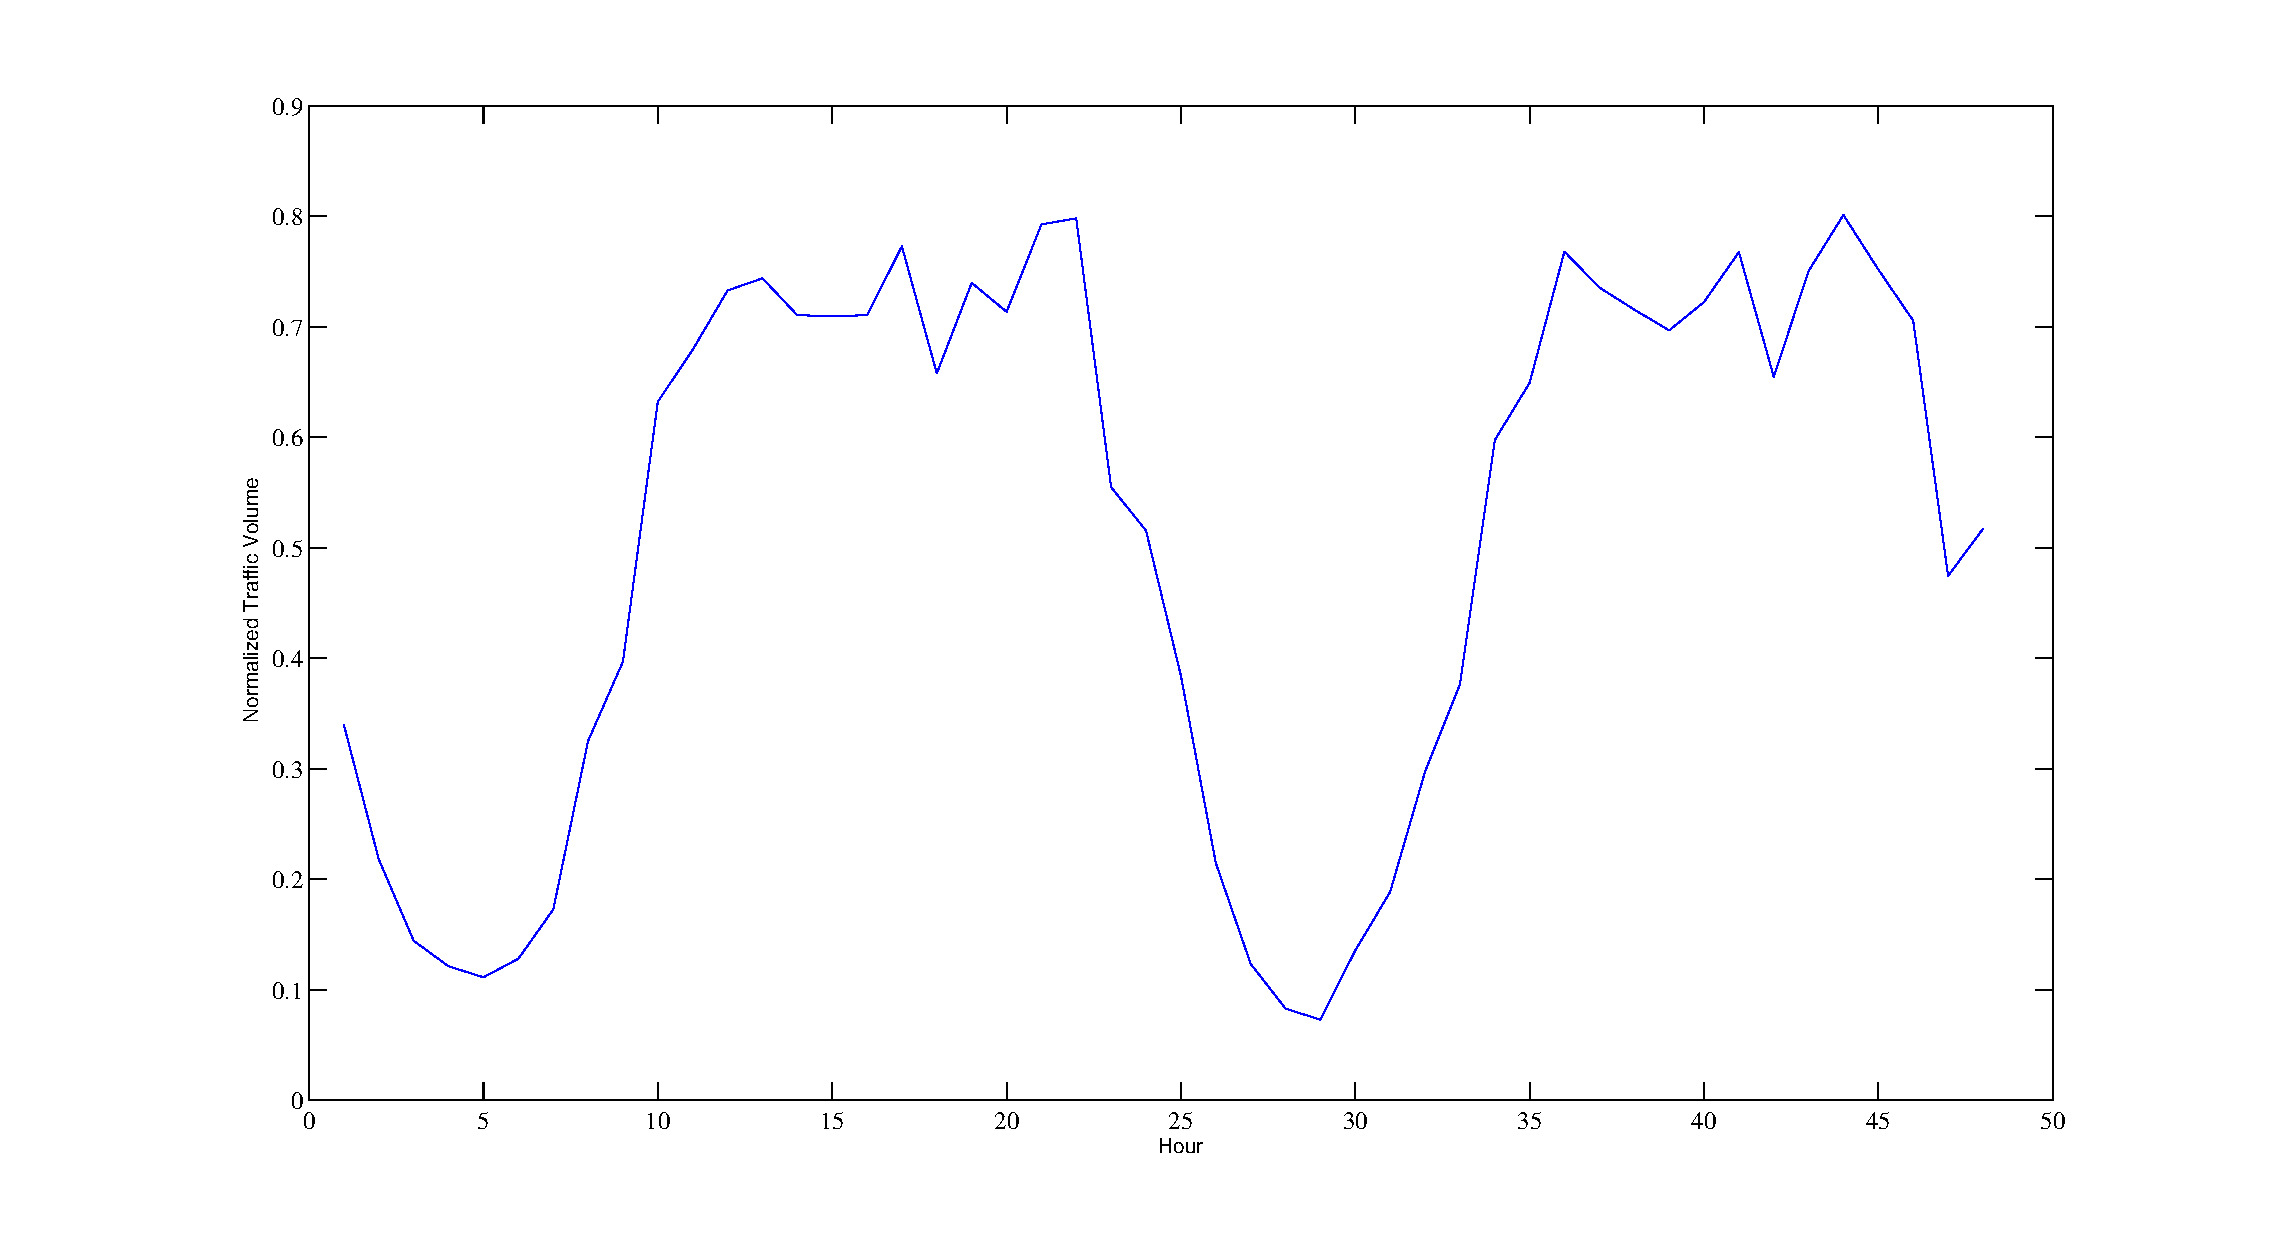
\includegraphics[width=0.7\textwidth]{pics/waridworkload.eps}
\caption{Call traffic for an operational cellular site over two days}
\label{fig:varwork}
\end{figure} 

\section{Prevalent electricity cost reduction techniques} %\textit{Electricity cost} = \textit{amount of energy consumed} $\times$ \textit{unit price of electricity}. Therefore, electricity cost may be cut by reducing either or both of the quantities on the right hand side. 

The electricity cost for a network is given by:
\begin{align}
\text{Electricity cost} = \text{amount of energy consumed} \times \text{unit price of electricity}
\label{eq:elec-cost}
\end{align}
Current work in reducing electricity cost for geo-diverse data centers and mobile cellular networks falls into two categories. The first category focuses on reducing the amount of energy consumed (thereby reducing the first term in equation~\ref{eq:elec-cost}), whereas the second category focuses on using cheaper sources electricity (thereby reducing the second term in equation~\ref{eq:elec-cost}). A taxonomy of the techniques that fall in these two categories is given in the next two sections.

\subsection{Reducing the amount of energy consumed}
\begin{enumerate}
\item \textbf{Hardware upgrades:} Due to ecological challenges, improved energy efficiency is generally a key requirement when developing new technologies and devices. For a given workload demand, an improvement in device energy efficiency lowers the amount of energy consumed, thereby reducing electricity cost. Therefore, hardware upgrades are a way to reduce electricity costs. An operator would, however, opt for hardware upgrades in their network only after they have obtained the Return on Investment (ROI) of the initial deployment or the end of life of deployed equipment. The initial investment not only involves capital cost of equipment but other factors such as spectrum licensing as well. In the cut-throat competition prevalent in most of today's networks, the ROI is slow to achieve. This means that existing energy inefficient networks would stay that way for a considerable time into the future.
\item \textbf{Hardware virtualization:} With the advent of ever faster CPUs, it was observed that servers tend to operate at relatively low CPU utilization most of the time. This was seen as an opportunity to statistically multiplex multiple servers onto a single physical machine by slicing the latter into multiple virtual servers. In this way, virtualization cuts capital costs for procurement of hardware. Since the virtual servers share the same resources (power supply, CPU, network interface, disks), if two servers are multiplexed onto a single physical server, the electricity consumption may be cut by as much as 50\%. A more aggressive server consolidation may cut electricity costs by upto 80\%~\cite{VirtualizationCutsPower}.
\item \textbf{Resource Pruning (RP):} Since network resources must be deployed according to peak demand while the workload peaks only for a short period of time, the excess resource may be deactivated (shutdown or put in power-saving mode depending on what is supported by the equipment) when the workload is low~\cite{Chase:2001:MES:502059.502045,Chen:2008:ESP:1387589.1387613,Meisner:2009:PES:1508244.1508269,Lin_dynamicright-sizing,Peng:2011:TPS:2030613.2030628}. When evaluating the reduction in electricity costs through resource pruning, it is imperative to consider any costs associated with activation and deactivation of network resources.
\end{enumerate}

\subsection{Using cheaper electricity - Workload Relocation (WR)}
Electricity prices exhibit geographic diversity~\cite{qureshiHotnets}, i.e., the price of electricity varies from one location to another. The variation in electricity price is generally noticeable only at large distances. For instance, the electricity price anywhere within a city is generally the same\footnote{With the exception of factors such as different tariffs for domestic, commercial and industrial consumers}. Most networks span large enough distances for geographic diversity in electricity prices to be apparent. 

If the network workload is quite flexible in terms of where it is handled, then the workload originating at a location with high electricity price may be relocated to a different location that has lower electricity price, thereby cutting the cost of electricity. We call this technique Workload Relocation (WR). 

Network workload exhibits varying levels of geo-flexibility. In geo-diverse data centers, for instance, the workload is highly geo-flexible, i.e., a client's request may be handled close by or even hundreds of miles away. On the other hand, the workload in cellular networks has very low geo-flexibility, i.e., a call must be handled at a cellular base station within a few hundred meters from the caller. Therefore, the amount of electricity cost savings achievable by exploiting geo-diversity in electricity prices through the use of WR is expected to be higher in data center networks than in cellular networks.

Electricity prices also exhibit temporal diversity~\cite{qureshiHotnets}, i.e., the relative order of electricity prices at different locations keeps changing. If a city in Kansas presently has cheaper electricity than one in Oklahoma, an hour later, the reverse may be true. This means that mapping of workload to locations must be periodically updated. The granularity of these updates depends on how frequently electricity prices change. Deregulated electricity markets, such as the ones in the USA, exhibit price changes at two different time scales (15 minutes for real-time electricity prices and an hour for day-ahead prices). 


\section{Our thesis} Based on the similarity in workload characteristics and the dependence of power consumption on workload, we opine that a generalized power optimization framework may be formulated that is applicable to many different types of networks. In this thesis, we focus specifically on geo-diverse data center networks and cellular networks. Our generalized electricity cost optimization framework would use workload relocation and resource pruning in tandem to reduce electricity costs\footnote{Hardware virtualization is complimentary to our framework}. 

\section{Contributions} This thesis makes the following contributions:

\begin{itemize}
\item We present a generalized model for electricity cost optimization applicable to different types of networks that jointly uses workload relocation and resource pruning. We show that this problem is NP-Hard.
\item We present a framework called Relocate Energy Demand to Better Locations (RED-BL), pronounced Red Bull, that solves the electricity cost minimization problem. We apply RED-BL to geo-diverse data centers as well as cellular networks using real data traces.
\item We obtain optimal solutions to RED-BL problems for both data center and cellular networks for realistic problem sizes. To handle the intractability of the problem, we also propose some heuristics that would be useful for even larger instances of the electricity cost minimization problem. 
\item Prior efforts in this area had mostly ignored the costs associated with activation and deactivation of network resources. To the best of our knowledge, we are the first to incorporate these in our optimization framework.
\item A network with significant over-provisioning may handle most of the workload at cheaper locations while the more expensive locations may be temporarily pruned from the network. In other words, geographic diversity in electricity prices incentivises over-provisioning. We study the benefits of increased over-provisioning and find diminishing returns with over-provisioning.
\end{itemize}

\section{Organization} The rest of the document is structured as follows. In Chapter~\ref{chap:background}, we compare two different types of networks and describe how similar they are in terms of workload handling and power consumption. In chapter~\ref{chap:framework}, we derive a generalized power consumption model, applicable to different types of networks and formulate RED-BL, a generalized electricity cost optimization problem. We present an evaluation of RED-BL on geo-diverse data centers and cellular networks in chapters~\ref{chap:casestudy1} and~\ref{chap:casestudy2}, respectively. In chapter~\ref{chap:conclusions}, we draw the conclusions and provide additional future directions.
\chapter{Background - Different Types of Networks and Their Similarities }
\label{chap:background}
In this thesis, we claim that many different types of networks are quite similar in terms of power consumption. In this chapter, we take an essentials-only look at two different types of networks with a view to establishing the similarity between them. This similarity motivates the formulation of a generalized electricity cost optimization framework. 

\section{Geo-Diverse Data Centers} Organizations like Microsoft, Facebook, Amazon and Google run a plethora of applications. Some of these applications are accessible by the general public. Google Docs is one such application. Such organizations also run private applications for the consumption of authorized internal users only. These applications run on servers that are hosted at sites called data centers.

A data center is a site that has equipment such as servers, storage and networking equipment, in addition to some allied equipment such as airconditioning and power supplies. A given data center may host only public applications, only private applications or even both. Furthermore, some public data center operators allow a client to host their own applications, whereas some only offer a fixed set of internally developed applications. For instance, one may run a custom application on a server leased on Amazon's data centers, but on the other hand, Google's search cluster only hosts the Google search application. 

Operators typically deploy multiple data centers at different geographic locations. This is done for two reasons. First, having data centers at different locations provides fault tolerance. If one site goes down for some reason, the other site may take over as a backup. Also, multiple remote sites are less likely to affected simultaneously by a natural disaster. A second reason to have multiple data centers is to have low latency to clients at different locations. For instance, Amazon has multiple data centers in different continents, thereby ascertaining that no matter where a client may be, there is an Amazon data center relatively close by compared to the case if Amazon only had one data center in the US. Figure~\ref{fig:googledcmap} shows the locations of Google's data centers across the globe (according to royal.pingdom.com as of April 2008).

\begin{figure}
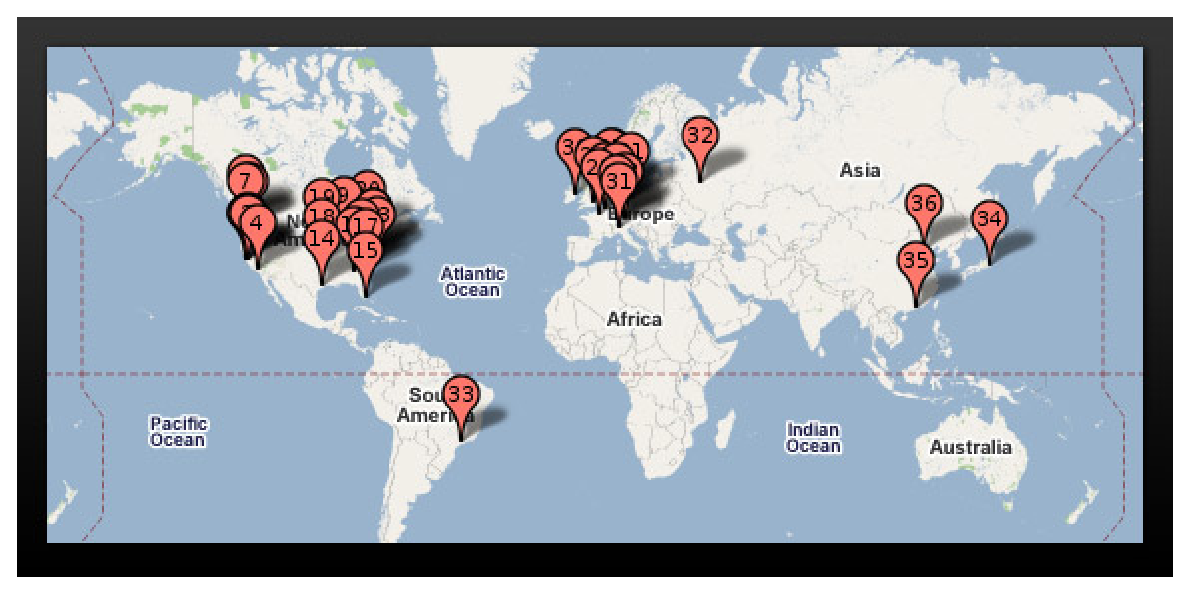
\includegraphics[width=1\textwidth]{pics/googledcmap.eps}
\label{fig:googledcmap}
\caption{Google Data Center Locations - Source: royal.pingdom.com}
\end{figure}
\subsection{Structure}
Before delving into the internal structure and composition of a data center, let us consider a data center as a single resource. This view helps provide only the high-level details of an operator's network. At this level, each one of an operator's data centers are inter-connected by means of high-speed inter data center network links. These links serve to carry various types of traffic, some of which are given below:
\begin{itemize}
\item \textbf{Consistency traffic:} To maintain consistency amongst replicas of an application's servers hosted in different data centers, some overhead in terms of network traffic must be incurred. For instance, a customer's website may be hosted at two different data centers and whenever a change is made to one copy of the website, the same changes must be reflected at the replica as well. 
\item \textbf{Traffic due to load-balancing:} Some traffic on the inter-data center links may be a result of the effort to achieve load-balancing amongst the data centers. For instance, the data centers may be oeprated by a web-based email service provider and the user inboxes may be partitioned over the data centers. In this case, an operator might desire that a roughly balanced amount of storage be used at each of the data centers. To this end, the operator might want to spread the inboxes over the data centers such that the cumulative size of the inboxes at each data center is roughly the same. Over time, due to changes in user behaviour and activity, the operator would need to re-adjust the inboxes assigned to each data center, thus requiring migration of inboxes between data centers. 
\item \textbf{Background traffic:} Yet another source of inter data center traffic is background traffic. For isntance, different data centers belonging to an Internet search engine operator may collaboratively compute search results. In this example, the search indices may also be updated periodically in the background.
\end{itemize}

\begin{figure}
\includegraphics[width=1\textwidth]{pics/dcheir.eps}
\caption{The modern data center's architecture}
\label{fig:dcheir}
\end{figure}

Having taken a high-level view of a geo-diverse data center operator's network, now let us delve into the internal structure and composition of a data center. Today's data center architecture is heirarchical~\cite{dcnetworking:vahdat:micro:2010} as shown in Figure~\ref{fig:dcheir}. A typical data center hosts tens of thousands of servers~\cite{Abts:2012:GTD:2184319.2184335}. The servers are installed in vertical racks. Apart from servers, the racks host other equipment as well. In addition to built-in hard drives in the servers, some dedicated storage nodes are also installed in the racks. A high speed Ethernet switch provides interconnection between the devices installed in the rack and connectivity to the rest of the data center and beyond. Power supply and distribution units for the equipment are also installed in the rack. 

A group of racks, called a pod (or a cluster), are interconnected by means of aggregattion switches. An aggregation switch allows servers in different racks to communicate with each other. All the pods within a data center are interconnected by core switches. This allows servers in different pods to communicate with each other. The core switches are interconnected through one or more border routers. These border routers are the avenues for traffic coming in and going out of the data center. 

All of the equipment is quite tightly packed within a pretty small space in a data center. The equipment generates a lot of heat and to prevent thermal damage to it, cooling must be provided. This is generally done by air-cooling, i.e., heat is transported away from the equipment by circulating cool air around it. 

\subsection{Request routing} 
%front-end server based load balancing and request routing mechanisms such as IP Anycast
As noted in chapter~\ref{chap:intro}, electricity cost depends not only on how much workload is handled, but also where it is handled. In order to develop a model for electricity cost in a geo-diverse data center, we need to first understand how workload from all over the globe is distributed amongst the data centers. In this section, we will use as an example a client request for viewing a web page hosted by a geo-diverse data center operator. 

To access a web resource, the user types a uniform resource locator (URL) in the web browser's address bar. The URL typically contains the DNS name corresponding to the web server that hosts the requested resource\footnote{It is also possible to specify the IP address of the web server directly in the URL. However, remembering IP addresses for all web sites of interest is not humanly possible}. Since a single server would hardly be sufficient to handle all traffic for a typical web site, several servers must be mapped to the same DNS name. However, the web browser must connect to exactly one of these servers during a browsing session. Figure~\ref{fig:dcloadbalance} briefly describes how this web server's IP address is picked. For details on DNS resolution process, see~\cite{rfc1034,rfc1035}. 

When the user enters a URL in her web browser, the browser invokes the local Domain Name System (DNS) resolver on the client machine which attempts to determine the IP address corresponding to the DNS name of the remote host specified in the URL. The local DNS server communicates with the DNS server for the client's ISP\footnote{Some people configure other DNS servers, such as Google's Open DNS Servers on their machines. In such cases, the local DNS server would communicate with the Google Open DNS Server}. The DNS query eventually reaches the authoritative server for the remote host's domain. In our example, this would be operated by the data center operator. The DNS server for the data center operator resolves the DNS name by returning an IP address corresponding to the DNS name specified by the client. The data center operator's DNS server performs an attempt at load-balancing so that roughly the same amount of workload is sent to each server hosting the requested web site. Notice in Figure~\ref{fig:dcloadbalance} that caches are available at various DNS resolvers in order to improve the latency of DNS resolution. These caches will keep the IP address corresponding to recently queried DNS names until the timeout specified by the authoritative DNS server expires.

\begin{figure}
\centering
\includegraphics[width=0.5\textwidth]{pics/dcloadbalance.eps}
\caption{Resolving the IP address for a server hosted in a data center}
\label{fig:dcloadbalance}
\end{figure}

The data center operator has a large pool of IP addresses, also known as IP address space, for their layer 3 devices. This IP address space is segmented over the geo-distributed data centers. The IP address resolved by the operator's DNS server belongs to one of the data centers and the client must now send it's Hyper Text Transfer Prototcol (HTTP)~\cite{rfc1945} request to the appropriate server at the corresponding data center. The client's web browser now establishes a Transport Control Protocol (TCP) connection with the server. To this end, the client sends packets to the web server's IP address that was just resolved. The packets leave the client's network interface and go to the ISP's gateway. Once in the ISP's network, the routers determine a path to the destination IP address and forward the packets hop by hop until the packets reach the data center where the required web server is hosted. 

Having determined the IP address of the web server, the client's web browser establishes an HTTP session with that IP address over a TCP connection. The IP packets belonging to this connection destined to the web server arrive at the border router in the corresponding data center and are forwarded to the server, traversing the core, aggregation and top of rack switches. The response packets are forwarded from the web server to the border router which routes it back to the client machine.

\subsection{Power consumption model} 
%Describe the power consumption model from prior work and derive a more simplified yet equivalent model
Fan et. al. used the results of a measurement study to show that the power consumption in a data center can be well-modeled as a linear function of the average CPU utilization~\cite{Fan:power:ICSA:2007}. As more and more client traffic arrives at servers in a data center, the average CPU utilization increases. If we consider homogenous client requests, the CPU utilization can be modeled as a linear function of workload. In case of heterogenous requests, one can approximate all request types as consisting of an integer number of micro-requests. Using the micro-request as our workload unit, we can still model CPU utilization as a linear function of workload. Since CPU utilization can be modeled as a linear function of workload, server power consumption can be modeled as a linear function of it's workload. The total power consumed by servers in a data center can, therefore, be represented as a linear function of the cumulative workload handled by the servers at the data center.


In our thesis, we wish to minimize the total electricity cost in a data center and servers are not the only power consuming equipment in a data center. Nonetheless, server power consumption is related to total data center power consumption by a measure called Power usage effectiveness (PUE). PUE is a measure of the efficiency with which a data center handles its power. It is defined as the ratio of total facility power to the IT equipment power. IT equipment power consumption includes power consumption by servers, storage and networking equipment. We assume that the power consumption in storage is related to that in servers, i.e., a unit workload consumes a fixed amount of power in storage devices. Networking equipment's power consumption is almost invariable with workload~\cite{Mahadevan:2009:PBF:1560132.1560210,Vishwanath:13,Chabarek08powerawareness}. Therefore, we can consider total IT power as being a constant multiple of server power consumption plus a constant amount (which is not important in our thesis since it plays no role in an electricity cost minimization problem). Therefore, PUE being a constant (depending on how efficiently data center is architected), data center power consumption is proportional to workload handled by the data center.

\section{Cellular Networks} %Just as data centers enable applications that we rely on every day, cellular networks are an important enabler of another pervasive service: telephony.
Being the older sibling of the Internet, telephony services are a more integral part of our every day lives than the Internet. Mobile telephone systems have enabled not only untethered access to traditional telephony services but also new types of services. We make phone calls, send text messages and can even connect to the Internet using our mobile phones. Just as Internet connectivity services are provided by ISPs and Internet applications are powered by data center operators, mobile phone services are provided by mobile network operators (MNOs).  

Over the years, mobile networks have been deployed based on different technologies. Literature often categorizes mobile network technologies in terms of \textit{generations}. First generation cellular networks (1G) were based on Advanced Mobile Phone System (AMPS). AMPS networks were deployed starting in 1978. The AMPS system also evolved into Digital-AMPS (D-AMPS) networks. Two technologies were part of the second generation (2G) cellular networks, namely Global System for Mobile communication (GSM) and Code Division Multiple Access (CDMA). Today, 90\% of the world's top 20 cellular networks use GSM technology~\cite{wiki:mobileoperators}. Anticipating the increased demand for mobile access to data services such as Internet access, vendors introduced General Packet Radio Service (GPRS) as an add-on to GSM networks. GPRS offers data rates between 56 kbps and 114 kbps. 2G networks with GPRS are sometiems referred to as 2.5G. GPRS bit rates are insufficient for many high bandwidth applications such as video calls, video streaming and video conferencing. To enable such services, broadband mobile services were introduced in third generation (3G) networks networks such as High Speed Downlink Packet Access (HSDPA) and Universal Mobile Telephone System (UMTS). The increasing trends in the use of high-bandwidth applications in mobile networks has spawned the fourth generation (4G) cellular networks such as WiMAX and Long Term Evolution (LTE).

\subsection{Structure} %A really basic introduction to cellular networks covering: concept of cells, mobile stations (MSs), Base Transceiver Stations (BTSs) and Base Station Controllers (BSCs)
In this thesis, as far as cellular networks are concerned, we focus specifically on GSM networks. Mobile phone networks are also referred to as cellular networks. The term cellular network stems from the fact that the area covered by the operator is logically divided into several small areas called cells. A cell in an urban setting (a macrocell) is typically upto a few hundred meters in radius, whereas in suburban or rural settings, the cell radius may be upto tens of kilometers. A \textit{cell site}, typically situated in the middle of a cell, enables subscribers in that cell to connect to the mobile network. A cell site is also often referred to as a Base Transceiver Station (BTS)\footnote{A single cell site sometimes hosts multiple BTSs, for instance, when multiple network operators share a single site} or simply a base station. A cell site hosts a number of transceivers (TRXs), radio antennas, power amplifiers and other allied equipment. 

Typically a government regulator such as Pakistan Telecommunication Authority (PTA) allocates a frequency band to each of the operators providing cellular service in the host country. The allocation is such that each operator gets a different frequency band. The spectrum allocated to a cellular operator is an integer multiple of the bandwidth of a single GSM channel (200 kHz). A cellular operator distributes their allocated frequencies to cells in their network. The channels allocated to an operator are much fewer than the number of cells in the network. Therefore, a given channel must be reused in an operator's network. Frequency reuse is done in such a way that any two cells that share the same frequency channel are sufficiently far apart so that the radio signal from any one of the cells does not noticably intefere with that in the other. In fact, each cell is typically divided into three sectors (resembling 120 degree pie-slices), therefore, the frequency allocation is done on a per-sector basis. Nonetheless, for a high-level view, the set of frequencies allotted to all sectors in a cell can be considered as allotted to the cell itself. Each TRX at a cell site operates at a distinct frequency.

Given two communicating parties at fixed locations, if the transmitted signal power is kept constant, the received radio signal strength would differ depending on the frequency used. Also, this frequency selective behaviour of the radio communication medium keeps changing with time, i.e., if frequency A receives better propagation compared to frequency B at time $t_1$, the same will not necessarily be true at time $t_1+\epsilon$. This means that we can't statically pick the best frequencies to use for a particular cell by considering, for instance, the type of terrain. In order to make decent communication conditions available to all callers, on average, GSM networks also use frequency hopping, whereby the frequency allocation to cells are changed periodically. 

To improve GSM's spectrum utilization, each frequency is also time-divided. For each frequency, a 120 ms duration transmission unit is called a GSM multiframe. It is named so because it consists of 26 frames of duration approximately 4.6ms each. Each frame is also divided into 8 bursts of duration approximately 0.577 ms each. The recurrence of a particular burst is what may be called a channel in GSM. In other words, a particular frequency and position within every frame defines a channel.

A MS often receives radio signals from multiple BTSs nearby. The MS picks the BTS from which it receives the strongest signal as it's serving BTS. A MS will do all communication such as call reception and placement through the serving BTS. When a subcriber moves around, the signal from the serving BTS might weaken. In such an event, the MS requests the network to allow it to change it's serving BTS to the one from which it currently receives the strongest signal. This is called a call handoff and is coordinated by a Base Station Controller (BDC).

Whereas a BTS is the access-side of a cellular, having no intelligence and performing only radio transmission and reception, the operations requiring intelligence such as frequency allocation, handoff coordination and frequency-hopping are controlled by a BSC. A BSC is responsible for several BTSs, which are connected to the BSC by means of some backhaul, such as E-1 or microwave links. A cellular network will typically have multiple BSCs, with a BSC being responsible for several BTSs in a vicinity. All BSCs are also interconnected by the cellular network's backbone, so that actions that require global coordination such as frequency assignment, frequency hopping and call handoff can be done smoothly.

Another key component of a GSM network is the Mobile Switching Center (MSC). The MSC is responsible for call routing both within the GSM network and beyond (to a landline phone, for instance). Since the focus of our thesis is power consumption in the network and 50\%~\cite{Louhi:2007:BTSPower:INTELEC} - 80\%~\cite{Oh:Comm:2011} of a cellular netowrk's electricity consumption is due to the BTSs, we will not dwell on the MSC and other components of the cellular network any more than necessary.

\subsection{Call placement} %How a call is handled by a BTS (at a very abstract level, i.e., how is the serving BTS chosen). Role of the BSC in cell association and call hand-off
For intelligible wireless communication, only one transmitter may transmit on a given frequency. Therefore, a call to/from a MS requires the allocation of two GSM frequencies, one for uplink (voice traffic from the MS to BTS) and the other for downllink (from BTS to MS). For coordinated acquisition of these frequencies, certain frequencies are reserved in each cell to serve as control channels. In fact, a caller does not get complete access to a particular pair of frequencies. Each of the 8 bursts in a GSM frame for a particular frequency may be used by different callers. Therefore, a particular frequency may be shared between multiple callers at a given time. In GSM terminology, they would all be using different channels, however, because a channel is characterized not only by the frequency but also the position within a GSM frame. Hence, the voice traffic for a call in GSM operates over two channels.

It appears that if $n$ frequencies are assigned to a particular sector, then it can support up to $8n$ simultaneous calls because that is the number of GSM channels available. However, this is not true for two reasons. 
\begin{itemize}
\item Some channels are reserved for control purposes. The exact number of such channels varies from operator to operator.
\item GSM supports two different types of codecs, namely the full-rate codec and the half-rate codec. The full-rate codec corresponds to a caller using a burst in every GSM frame during a call, whereas the half-rate codec corresponds to a caller using a burst in every alternate GSM frame. By default, the full-rate codec is used for every call. However, when traffic congestion rises above an operator-configured threshold, the network attempts to admit every new call using a half-rate codec, if the corresponding MS supports it. If the traffic rises further and crosses a second threshold as configured by the operator, the network also re-assigns current calls to use a half-rate codec depending on the corresponding MS support. This enables a BTS to support more than $8n$ simultaneous calls during times of congestion.
\end{itemize}
 

\subsection{Power consumption model} %Describe the power consumption model from prior work
BTSs account for most of the power consumed in a cellular network. \cite{Louhi:2007:BTSPower:INTELEC} claims that BTSs contribute 50\% of overall network power consumption, whereas~\cite{Oh:Comm:2011} puts this number at 80\%. For this reason, most of the prior work related to power consumption in cellular networks focuses on BTSs. 

Lorincz et. al. performed a measurement study of BTS power consumption under real-traffic conditions and concluded that the power consumption may be approximated as a linear function of call traffic~\cite{Lorincz:BTS-Measure:Sensors:2012}. Thus, as traffic varies during a given day, instantaneous power consumption would follow a similar curve as the traffic.

\section{Similarities between different types of networks} %Geo-diverse data centers and cellular networks are similar in the sense that both are built out of network resources to handle workload which results in electricity consumption. 
From our discussion of two different types of networks, we can see that they are both essentially a collection of interconnected sites (data centers and BTSs) which are a collection of resources (data centers and TRXs). The workload in both types of networks exhibits diurnal patterns~\cite{10.1109/MC.2007.443,Peng:2011:TPS:2030613.2030628}. The network in both cases is provisioned according to peak workload demand. Since the network resources are not energy proportional, this means that in low-workload regimes, the network is heavily over-provisioned. The resulting energy inefficiency can be dealt with by deactivating some resources when the traffic is low.

In terms of power consumption also, the two networks considered in this chapter, namely geo-diverse data centers and cellular network are quite similar. Both have a linear mapping from workload to power consumption. This motivates the possibility of establishing a common framework that smartly schedules the network resources in response to workload variations so as to minimize electricity costs.

\section{Differences between different types of networks}
All characteristics of different network types are not essentially similar. Several attributes are different as well. The following list summarizes some differences between geo-diverse data centers and cellular networks

\begin{itemize}
\item \textbf{Workload granularity:} The workload capacity of a data center is very large, potentially in millions of client requests per second, whereas the workload capacity of a TRX is less than eight simultaneous calls. For this reason, instead of determining the exact integer number of requests to handle at each data cneter, the fraction of workload to be handled at each data center can be determined as a real-number (which is a much simpler problem to solve), and the resulting number of requests will most likely be an integer or may be rounded off with little change in electricity cost. Meanwhile, in case of cellular networks, the cumulative workload for a cell is a small number of calls and each call must be handled at exactly one of a few candidate cells. Hence, the call to cell mapping must be binary in nature and fractional mapping algorithm will not work.
\item \textbf{Geo-diversity in electricity prices:} In a geo-diverse data center scenario, the network resources, i.e., data centers are quite far from each other and hence electricity price differential due to geo-diversity in electricity prices is quite likely. However, in case of cellular networks, the cell sites are within a few hundred meters of each other (in an urban setting) and an electricity price differential is highly improbable. 
\end{itemize}



\chapter{A generalized framework for electricity cost optimization}
\label{chap:framework} In Chapter~\ref{chap:background}, we observed that there are several similarities and a few subtle differences between geo-diverse data center and cellular networks in terms of their power consumption models. We proposed a generic view of geo-diverse data centers and cellular networks as a collection of resources that are used to handle client workload. We also saw that their power consumption may be modeled as an affine function of the amount of workload handled. In this chapter, we will use this generic model to formulate a generic optimization problem that minimizes electricity cost for both these networks. Our generic power consumption model and the corresponding electricity cost optimization problem incorporates the subtle differences, as discussed in section~\ref{sec:chap2:comparison}, between the data centers and cellular networks.


\section{Optimization Problem Model} %Discuss how different network types can periodically use RP and WR to minimize electricity costs. Show that this problem is NP-Hard. Describe the concept of network state and motivate a state trajectory optimization problem. Describe transition costs and formulate a mathematical optimization problem.
In order to develop a generalized optimization problem for minimizing electricity cost, we use an illustrative example shown in Figure~\ref{fig:mappingexample}. The example uses a test tube to represent a network resource and marbles to represent a unit workload. The network resource would be a data center in the context of geo-diverse data center operator, whereas it would be a BTS in the case of a cellular operator. Similarly, the workload unit would be a client request in the data center context, whereas it would be a call in a cellular network setting. The operator's goal is to assign workload to network resources and, if needed, periodically update this assignment in response to variations in workload.

\begin{figure}
\centering
\includegraphics[height=0.8\textheight]{pics/mappingexample.eps}
\caption{An example of mapping variable workload to capacity-limited network resources with geo-temporal diversity in electricity prices. Three consecutive intervals $t_1$, $t_2$ and $t_3$ are considered. Workload and electricity prices may only change between two consecutive intervals. (a) Workload considered in this example. (b) Electricity prices for the locations at which the two network resources are situated. (c) A uniform mapping of workload to network resources does not exploit electricity price diversity. (d) Mapping workload to network resources in order of their current electricity price. Due to lack of energy proportionality, only slight savings in electricity cost are possible. (e) Deactivating idle resources alongwith the resource mapping strategy of (d) may result in significant electricity cost savings.}
\label{fig:mappingexample}
\end{figure}

We consider the largest possible quantum of time for which the workload (and electricity price) remains fixed and term each such quantum as an \textit{interval}. We assume that workload for several consecutive intervals is known and term this sequence of intervals as a planning window. The example in Figure~\ref{fig:mappingexample} demonstrates three different ways (shown in parts c, d and e) of mapping this workload to two network resources situated at different locations over a planning window consisting of three intervals centered at $t_1$, $t_2$ and $t_3$. In each interval, we assume that the workload is geographically split such that half of it originates near each of the two resources. For this example, we consider temporal variation in workload as shown in Figure~\ref{fig:mappingexample} (a). Meanwhile, Figure~\ref{fig:mappingexample} (b) shows the geo-temporal variation in electricity prices for the two network resources.

One possible operational strategy is to map each workload unit to the nearest available resource as shown in Figure~\ref{fig:mappingexample} (c). In a sense, this is the default strategy in cellular networks, whereby a call is handled by the BTS from which the mobile station (MS) receives the strongest radio signal\footnote{Signal from the physically nearest BTS may be weakened considerably due to natural or man-made obstructions. In such cases, the nearest BTS may not be the one from which the strongest signal is received. Hence, we take "nearest" to mean the BTS from which the MS receives the strongest signal}. In geo-diverse data center settings, this mapping strategy is also often the default strategy because it minimizes the access latency for all clients\footnote{Network latency has been shown to have a strong correlation with the physical shortest path distance between two locations on the globe~\cite{dina:p2pdelay:infocom:2004}. So, the commonly understood physical measure of "shortest" applies in this case.}. 

The above workload-resource mapping strategy pays no attention to geo-diversity in electricity prices. We can exploit geo-diversity in electricity prices to reduce the electricity cost over the planning window by mapping more workload to resources at cheaper locations. To this end, we must change the way workload is mapped to resources as the electricity prices at various locations change. We term such changes in workload-resource mapping as Workload Relocation (WR). 

Figure~\ref{fig:mappingexample} (d) shows a mapping strategy that uses WR to map as much workload as possible to resources at cheaper locations. In interval $t_1$, since the cumulative workload equals the total network capacity, both network resources will be operating at full capacity. Accordingly, there is no opportunity to reduce electricity costs using WR or RP. In interval $t_2$, on the other hand, as shown in Figure~\ref{fig:mappingexample} (d), we may use WR to move all workload to network resource B, which is situated at the location with the cheapest electricity price, thereby reducing electricity cost for that interval as compared to the default workload-mapping strategy. Similarly, in interval $t_3$ WR may be used to shift workload such that the cheaper resource A is loaded to full capacity and the remaining workload is mapped to the other resource. 

Due to lack of energy proportionality in networks, the power consumption of idle resources is a large fraction of their peak power consumption. Hence, consolidation of workload to cheaper locations offers a limited benefit in terms of reducing electricity cost compared to the default workload-mapping strategy. To avail considerable savings in electricity cost, one must use resource pruning (RP), i.e., deactivate idle resources. Notice that in the default workload-resource mapping strategy of Figure~\ref{fig:mappingexample} (c), there is no opportunity to deactivate idle resources in any of the three intervals. However, the purely-WR strategy of Figure~\ref{fig:mappingexample} (d) may be augmented with RP, as shown in Figure~\ref{fig:mappingexample} (e), to achieve maximal savings in electricity cost. The strategy in Figure~\ref{fig:mappingexample} (e) not only shifts workload to the cheapest possible resources, but also deactivates as many resources as possible. 

In claiming that Figure~\ref{fig:mappingexample} (e) shows the maximal savings in electricity cost, we have assumed that activation and deactivation of network resources is free of cost. However, such costs may exist in practice and in some networks it may even be significant compared to the total electricity cost of network operation. In such cases, care must be taken when defining the optimal strategy for network operation. %With this in mind, we draw parallels with similar problems in other domains with known results on optimal solutions and hence draw conclusions on the computational complexity of the optimal electricity cost network operation.

Unused fractions of a network resource continue to consumer power on idle. Electricity cost savings from the WR and RP strategies may be improved if unused fractions of network resources could be deactivated. For instance, if a data center is running at 50\% of its capacity in a given interval, half of it might be deactivated. In our example of Figure~\ref{fig:mappingexample} (e), in intervals 2 and 3, half of resource B might be deactivated. 

%\subsection{Problem complexity}
%\label{subsec:framework:complexity}
%During each interval, the network operation problem maps to the multiple knapsacks problem ~\cite{kellerer:knapsackproblems:2005,Chekuri99aptas}, whereby a subset of a given set of items, each with a certain weight, must be selected and placed into several weight-limited knapsacks such that the total profit from the selected items is maximized. Since the single-interval instancce of our problem is analogous to the multiple knapsacks problem, which is known to be NP-Hard~\cite{kellerer:knapsackproblems:2005,Chekuri99aptas}, each single-interval instance of our problem is NP-Hard as well. Hence, the multi-interval planning problem must also be NP-Hard. This applies to cellular networks, for instance, where every call may be associated to exactly one BTS. 
%
%In certain type of networks, workload may be fractionally distributed, i.e., the cumulative workload during interval $j$, denoted $x^j$, may be distributed amongst the network resources such that each network resource gets a fraction of the workload dentoed $x_i^j$. In such networks, the sum of $x_i^j$ over all network resources must equal $x^j$. As discussed in section~\ref{sec:background:differences}, workload mapping in geo-diverse data centers may be approximated using such a scheme\footnote{The number of client requests per interval is so large that the fractional distribution (to a reasonable precision) of workload amongst resources results in a solution that will most likely have an integer number of requests mapped to each data center}. One would expect that the resulting problem would be simpler to solve and shouldn't be NP-Hard, because the single interval instance now resembles the fractional knapsack problem which may be solved optimally using a greedy strategy. But as we shall see, when RP is applied in a multi-interval setting, even this version of the problem is NP-Complete.
%
%We compare this second version of our problem to the unit commitment problem~\cite{unitcommit-trans} in distributed electricity generation and distribution scenario, which is known to be NP-Complete. The unit commit problem determines the generation levels of several power generating resources, given time-varying demand for electricity that may be derived from any of the active generating resources in any fraction. The generating resources may be turned off when electricity demand is lower than the cumulative capacity of running generating resources while incurring a ramp-down cost. Similarly, a generating resource may be turned on when demand exceeds the capacity of resources that are currently operating while incurring a ramp-up cost. Ramp-up and ramp-down costs as well as costs of generating a unit of electricity at each generating resource depends on the fuel prices at the location where the corresponding generating resource is situated. Furthermore, a generator is allowed to run on no-load as a spinning reserve while incurring idle fuel costs. If we represent the time-varying electricity demand as the network operator's workload and replace the generating resources by data centers, we have a one-to-one mapping of the unit commit problem to our geo-diverse data center scenario. Since the unit commitment problem is NP-Complete, it follows that so is the fractional workload-mapping version of our problem.

\section{Optimization problem formulation}
\label{sec:framework:optimization}
On a high-level, routine network operation involves distributing workload to network resources and periodically updating the fraction of workload mapped to each network resource. For simplicity of modeling and analysis, we assume that the mapping of workload to network resources, henceforth referred to as \textit{workload mapping} or simply \textit{mapping}, is updated at the beginning of intervals of fixed duration. We denote the status of resource $i$ during interval $j$ by $p_i^j$, which may be a binary variable if the resource may be either active or inactive. It may be possible to configure a resource at a finer granularity, and thus, in general, $p_i^j$ may have a value between $0$ and $l$. We denoted the workload being handled by resource $i$ during interval $j$ as $x_i^j$. We refer to the status and amount of workload mapped to resource $i$ at time $j$ collectively as the resource's state, denoted $s_i^j$. The aggregated state of all network resources during interval $j$ may be termed as the \textit{network state} during the corresponding interval, denoted by $S^j$. The routine network operation can thus be modeled as determining a sequence of network states for a time horizon, called a \textit{planning window}, consisting of a set of consecutive intervals of equal duration. In the context of our thesis, the objective is to determine the state trajectory that is optimal in the sense that it minimizes the electricity cost over the planning window. %The interval after which the workload mapping may change need not be less than the interval during which the workload and electricity prices remain almost constant. Both problems, i.e., mapping real fractions of workload to network resources (as in the geo-diverse data center scenario) and the 0/1 mapping of workload (as in the cellular network scenario) are multi-interval allocation 

\subsection{The objective function}
\label{subsec:framework:objective} %Provide the mathematical form of the objective function that is designed to solve the optimal state trajectory problem.
The optimal state trajectory problem attempts to determine a sequence of states such that the sum of state costs and the cost of transitions between states in consecutive intervals is minimized. Mathematically, we may present the objective function as:

\begin{align}
\sum_{j=1}^n C(S^j) + T(S^j, S^{j-1})
\end{align}

Here $C(S^j)$ represents a function that evaluates the cost of being in state $S^j$. As per equation~\ref{eq:abdcpaper}, $C(S^j)$ may be given as:
\begin{align}
C(S^j) = \sum_{i=1}^m \left\{ P_{min} + x_i^j (P_{max} - P_{min}) \right\}
\end{align}

Furthermore, $T(S^j,S^{j-1})$ represents a function that computes the cost of transitioning from state $S^{j-1}$ to state $S^j$ during consecutive intervals $j-1$ and $j$. The transition costs may be a result of factors such as overhead electricity consumption when turning network resources on or off. We will show in the next chapter that transition costs can be computed using the values of the indicator variables $p_i^j$ and $p_i^{j-1}$.

\subsection{The constraints}
\label{subsec:framework:constraints} %Comment on some of the network-specific constraints that the optimization must be subject to.
The state trajectory problem must be subject to a number of problem-specific constraints. Some constraints are common to both geo-diverse data centers and cellular networks. 

\begin{itemize}
\item \textbf{Resource capacity must be respected:} During all intervals, we must ensure that the workload mapped to each network resource does not exceed its capacity.
\item \textbf{All workload must be handled:} During all intervals, the sum of workload mapped to all network resources must equal the offered workload for that interval.
\item \textbf{Network resource status is binary:} The status of a network must be represented as a binary variable which takes on the value 1 if the said network resource is on during a given interval, and 0 otherwise. It might appear that the resource status is redundant given that we are also keeping track of the workload mapped to the resource as part of its state. After all, if the workload mapped to a resource is $0$, it can be considered off and considered on if the workload is greater than $0$. However, there is no linear function that can calculate cost of resource activation and deactivation given the workload mapped to the resource in two consecutive intervals. One must introduce an auxiliary variable that represents resource status in order to keep the optimization formulation linear\footnote{Introduction of non-linearity in an optimization problem increases its computational complexity.}. 
\end{itemize}

Several network-specific constraints must also be formulated. These constraints arise from subtle differences between different types of network. For instance, while any client request can be handled at any data center, a given call may be handled by only a few BTSs that are in the immediate vicinity of a caller. Such constraints will be specified in later chapters.

\subsection{Comments on the problem formulation}
The decision variables in our problem formulation are the state of network resources for each interval in the planning window. A resource's state has two parts: the amount of workload it handles and its status (on or off). The resource status needs to be a discrete (binary) variable. The amount of workload may also be a whole number in some network types. For instance, in a cellular network context, the workload mapped to a resource represents the number of active calls being handled by a BTS, which is a whole number. It is also possible to formulate the problem such that the workload mapped to a resource during an interval is represented as a fraction of the operator's total workload during that interval. In the first formulation, the resource state is purely discrete, whereas in the second formulation, the resource state is composed of a discrete as well as real-valued parts. In the former case, our optimization problem is an integer program (IP), whereas in the latter, the problem is a mixed integer program (MIP). Both IP and MIP are NP-Hard and must be solved using techniques such as branch and bound~\cite{land60a} or other heuristics. 

If functions $C(.)$ and $T(.,.)$ as well as all constraints are linear and convex, the formulation is termed as an integer linear program or mixed integer linear program. Since the branch and bound technique repeatedly solves constrained and integer-relaxed versions of the IP (or MIP), linearity of the objective functions lowers the computational complexity. Fortunately, the nature of energy consumption in networks is such that the power consumption function $C(.)$ is linear and convex. For this reason, in our thesis, we strive to make the transition cost function $T(.,.)$ as well as all problem constraints as linear.

In this chapter, we have presented an abstract formulation of the general optimization problem for minimizing electricity cost in service provider networks. Two concrete instances of the optimization problem are discussed in the next two chapters. In order to solve both of those concrete instances, we used the CPLEX solver available with the ILOG CPLEX Studio. CPLEX solver uses the branch and bound heuristic. Our primary focus in this thesis is to investigate the potential that the use of RP and WR offers for electricity cost optimization. Therefore, we focus on solving both concrete instances of the optimization problem \textit{exactly}. As we shall see in the next two chapters, we were able to solve problems of reasonable size using simple desktop PCs within a reasonable amount of time. While our primary focus is not on proposing heuristics for approximate solutions to the problem, in the next two chapters, we do propose an approximation algorithm for the optimization problem for each of networks considered in this thesis. 
\chapter{Case Study I: Geo-diverse Data Centers}

\section{Instantiating the generalized optimization formulation} Derive the objective function and constraints. Clearly outline the assumptions that we've made about the geo-diverse data centers.

\section{Experimental Setup} 

\section{Results}
\subsection{Sensitivity of electricity cost savings to extent of overprovisioning}
\subsection{Sensitivity of electricity cost savings to extent of geo-diversity}
\subsection{Sensitivity of electricity cost savings to magnitude of transition costs}
\subsection{Sensitivity of electricity cost savings to resource pruning granularity}
\subsection{Sensitivity of electricity cost savings to workload estimation errors}
\subsection{Sliding window re-optimization}

\section{Discussion}
\chapter{Case Study II: Cellular Networks}
\label{chap:casestudy2}
\section{Prelude}
Cellular networks consume several tens of TWhs (terawatt-hours) of electrical energy worldwide every year~\cite{Oh:Comm:2011}, exacerbating rising ecological concerns. Beyond these concerns, the corresponding cost of electricity makes up a significant proportion of the overall operational cost of a cellular service provider.
In European markets, for example, the electricity cost is
estimated to be around 18\% of the operational costs~\cite{Blume:2010:BLTJ:CellularPower}.
This fraction is even higher in developing regions due to the shortage of grid electricity and the use of small-scale generation powered by diesel fuel. Thus, cellular operators are keen on reducing the power consumption of their networks.

In this chapter, we discuss RED-BL's application to save energy in cellular networks. To this end, we utilize \textit{Base
Transceiver Station (BTS) Power Savings} and \textit{Call
Hand-off} to reduce the BTS power consumption. Using deployment
and traffic data from a cellular provider in a large metropolitan area in a developing region, we show that
RED-BL can save about 10\% in the amount (and cost) of electrical energy.
This translates into millions of dollars in annual savings, just for this one service provider.


RED-BL achieves this saving in energy consumption by reducing the power consumption at BTSs, which account for 60\% to 80\% of a cellular network's total power consumption~\cite{Oh:Comm:2011,Louhi:2007:BTSPower:INTELEC,Peng:2011:BTSSaving:Mobicom}, by making them more energy proportional.
Figure~\ref{fig:workload-variation} shows the normalized load of consumer traffic at two neighboring BTSs in our dataset.
Observe that while the traffic load peaks for a short period of time, it mostly stays at a fraction of its peak\footnote{Operational cellular networks have been widely observed to exhibit traffic load variations both over time and space \cite{Peng:2011:BTSSaving:Mobicom}.}.

However, the radio circuitry at BTSs is provisioned in accordance with the peak load.
This radio circuitry lacks energy proportionality i.e., its power consumption does not scale in proportion to the traffic load.
As a result, a BTS also lacks energy proportionality and consumes power at about the same level as it would at the peak load~\cite{Peng:2011:BTSSaving:Mobicom}. This leads to wasted energy, which RED-BL aims to reduce---by varying the power consumption at a BTS in accordance with its traffic load.

\begin{figure}[t]
\centering
\includegraphics[width=0.8\textwidth]{pics/ilyas1.eps}
\caption{Traffic load variations at two neighboring BTSs during a single day from our dataset. For most of the day, the instantaneous load is a fraction of the peak traffic load.}
\label{fig:workload-variation}
\end{figure}


If the instantaneous power consumed at a BTS can be made proportional to the instantaneous
workload, savings in power consumption will ensue.
For the provider data available to us, a fully energy proportional BTS subsystem of a cellular network would save between $44\%$$-$$52\%$ of electrical energy depending on the BTS model.
Thus, there exists potential to save electricity cost in a cellular network by reducing the energy consumption at low workloads.
RED-BL exploits this potential in two ways: (i) \textbf{Resource pruning}: shutting down part of the radio circuitry, and (ii) \textbf{workload relocation}: rerouting calls from one BTS to a nearby BTS.

 
Coarse-grained energy proportionality in BTSs may be achieved in one of the following two ways:
\begin{itemize}
\item BTSs may be turned off when traffic is low and turned on later when traffic load
increases~\cite{Oh:TWC:2013,6503647,Oh:Globecom:2010,5208045,Oh:Comm:2011,marsan:wgreen:2008}.
However, operators are often reluctant to switch on/off entire BTSs due to coverage and equipment lifetime concerns.
\item \textit{Frequency dimming}~\cite{Tipper:Dimming:Globecom:2010} proposes to turn off a fraction of
the radio circuitry when traffic is low, such that the traffic may be handled by the circuitry that stays on.
Most vendors' BTSs support such a feature, which we term as \textit{BTS power savings} in this paper.
Our conversations with cellular operators reveal that they regularly use this feature. RED-BL also makes use
of this feature.
\end{itemize}

The novelty in our approach is that we couple BTS power savings with call hand-offs to increase the
energy savings possible through BTS power savings alone. While call hand-off is commonly used to
reduce mobile station (MS) transmitted power, to the best of our knowledge, our work is the first to exploit call hand-offs for reducing BTS power consumption.

Traffic traces collected from a large network operator indicate that if some calls are handed off between
neighboring BTSs, the number of BTSs that can be put in BTS power savings mode can be increased.
Thus, RED-BL proposes to hand-off calls between neighboring BTSs, without making a negative
impact on the network quality of service, such that the \textit{BTS power savings} can be applied to a
maximal number of base stations throughout the cellular network. In comparison to uncoordinated \textit{BTS power savings}, as used in current cellular network deployments, RED-BL
offers additional power savings as it may allow a larger number of radio circuits to be deactivated.

The underlying assumption in RED-BL is that calls can be handed off to neighboring BTSs
without being dropped and without exceeding their traffic capacity. This is possible because (a) traffic load in cellular networks exhibits significant variation over time and space and (b)
most callers often receive sufficiently strong signal from \emph{several} nearby
BTSs~\cite{Peng:2011:BTSSaving:Mobicom,lowcarb:2013:globecom}.
This coverage diversity is evident in Figure~\ref{fig:btscdf}, which shows the CDF of the number of BTSs available to an end-user in our dataset of live traffic.
Observe that the results show that about half of the callers have 3 or more candidate BTSs available at all times
Thus, some calls may be handed off from one BTS to a nearby BTS in order to increase energy savings over those
possible through BTS power savings alone.
\begin{figure}[h!]
\centering
\includegraphics[width=0.8\textwidth]{pics/ilyas2.eps}
\caption{Cumulative distribution function (CDF) of the number of potential serving BTSs for a call in our dataset (large metropolitan area).}
\label{fig:btscdf}
\end{figure}

During low traffic periods, network operators often use a feature available in most vendor's equipment that deactivates TRX circuits at locations that
serve very few customers. Huawei calls this feature \textit{TRX shutdown} while Ericsson calls it \textit{BTS power savings}. We use the latter term generically in this paper. Turning off one TRX cuts down BTS power consumption anywhere from $20W$
to $100W$, depending upon the frequency band (900 or 1800) and
deployed
equipment~\cite{Lorincz:BTS-Measure:Sensors:2012,flexibsc}.
Thus, scaling a ``6+6+6'' to a ``2+2+2'' configuration, by deactivating 12
TRXs will result in a saving of
240W to 1200W on a single site.

\subsection{Motivating example}

\begin{figure}
\centering
\includegraphics[width=0.6\textwidth]{pics/ilyas3.eps}
\caption{The scenario for the motivating example. Three BTSs (A, B and C) are shown along with eight active calls. Each call is handled by the BTS from which it receives the strongest signal (the default in GSM networks). The serving BTS for each call is shown using arrows. If the power savings mode can be enabled at a BTS that has up to two active calls, then only BTS C can be put in the power savings mode. However, if calls 7 and 8 were handed off to BTS C, both BTS A and B can be put into the power savings mode, thereby resulting in greater energy savings.}
\label{fig:illustrationall}
\end{figure}

\begin{table}
\centering
\begin{tabular}{|c|c|c|c|c|}
\hline
Scheme & \multicolumn{3}{|c|} {Calls being handled by BTSs} & BTSs in power \\
\cline{2-4} \ & A & B & C & saving mode \\
\hline Default & 1, 2, 7 & 3, 4, 8 & 5, 6 & None \\
\hline Power saving & 1, 2, 7 & 3, 4, 8 & 5, 6 & C \\
\hline RED-BL & 1, 2 & 3, 4 & 5 -- 8 & A, B\\
\hline
\end{tabular}
\vspace{+0.1in}
\caption{A comparison of schemes for BTS power savings}
\label{tab:example}
\end{table}

To illustrate the working principle of RED-BL, we consider an example deployment consisting of three BTSs serving eight calls in neighboring cells as shown in Figure~\ref{fig:illustrationall}.
By default, each call is served by the BTS from which the mobile station receives the strongest signal. Assume that each BTS may handle up to six simultaneous calls and that the power-saving threshold is two calls, i.e., a BTS serving up to two calls may be put into power-saving mode.

The first row in Table~\ref{tab:example} indicates that under default call association, no BTS in the example deployment of Figure~\ref{fig:illustrationall} is placed in power saving mode.
With this default call association, the operator may still save some electrical energy by activating the power saving mode on BTS C (second row in Table~\ref{tab:example}).
Additional energy savings are possible by deploying RED-BL, which hands off calls 7 and 8 to BTS C and enables power saving mode on two BTSs (A and B), as shown in the third row in Table~\ref{tab:example}.


This example shows that the current practice of enabling power savings mode based on traffic conditions that are local to a BTS can result in sub-optimal energy savings.
RED-BL achieves greater energy savings by jointly using call hand-off and BTS power savings.

\section{Related work}
\label{sec:related}

In~\cite{Peng:2011:BTSSaving:Mobicom}, the authors proposed that when the traffic in an area being served is low, the serving BTS may be completely turned off to save power. Later, when the traffic volume rises, such BTS may be turned on again. To avoid lack of coverage when a BTS is turned off, its neighboring BTSs must, however, increase their transmit power.
Similar proposals are also reported in~\cite{Oh:TWC:2013,6503647,Oh:Globecom:2010,5208045,Oh:Comm:2011,marsan:wgreen:2008}. Moreover, conversations with operators indicate that they are reluctant to turn off entire BTSs due to reduced expected lifetime of the installed electronic equipment.

\textit{Frequency dimming}~\cite{Tipper:Dimming:Globecom:2010} proposes to turn off some TRXs on a BTS when the traffic is low. RED-BL goes beyond frequency dimming --- it reroutes the calls and can potentially enable power savings mode on a larger number of BTSs.
Coarse estimates of the energy saving potential of TRX deactivation were presented
in~\cite{Blume:2010:BLTJ:CellularPower}.
In contrast, we use site locations and real traffic traces from a large cellular network with more than 13 million subscribers to run a simulation study assessing the benefits of dynamic equipment scaling coupled
with call hand-offs. Note that BTS power saving represents RP in the RED-BL framework whereas call handoff represents WR.

There exists a large body of work on solutions to constrained resource optimization problem, like the one we formulate for RED-BL. For example, such problems have been addressed in the context of data centers~\cite{Jeyarani:2012:DIA:2148243.2148374,serverEnergy,Mazzucco:Maximizing:2011:CoRR,Oh:2011:ECS:2170444.2170458,Chase:2001:MES:502059.502045}, scheduling in compute clusters~\cite{AlDaoud2012745}, System on Chip (SOC)~\cite{Fang:2011:COP:1995896.1995940}, electric power systems and smart grids~\cite{Javed:2008:ULP:1485753.1485792,Logenthiran2011138,Celli:2001:PICA,FahadJavedAdOpt.SASO.2009.26}, WiFi access points~\cite{Marsan:2010:SAM:1791314.1791340}, wide area networks~\cite{Cavdar:2011:ECOC} and high performance computing~\cite{Lee:ServerConsolidation:2011:Globecom,Pinheiro01loadbalancing,Yao:DCPowerReduction:2012:INFOCOM,Herodotou:Starfish:2011:CIDR,Herodotou:2011:NOS:2038916.2038934,Aikema:ElecCostHPC:2011:ISSST}.




\section{Instantiating the generalized optimization formulation} %Derive the objective function and constraints. Clearly outline the assumptions that we've made about the geo-diverse data centers.
\label{sec:case2:instantiate}
The RED-BL optimization problem minimizes the sum of state and transition costs for a network over a sequence of consecutive intervals in a planning window. The state cost for a particular interval is the sum of electricity cost incurred at all BTSs in the network. In order to compute the state cost, we will first derive a mathematical model for electricity consumption at a single BTS. Then, we will generalize it to a multi-BTS cellular network setting to represent the state cost for a single interval. The transition cost would be the cost of electricity incurred in activating or deactivating TRXs. Our conversations with network operators reveal that transitions into and out of BTS power saving mode do not consume a noticeable amount of power. These state transitions are reasonably fast in contrast to the delayed convergence due to transitions in the geo-diverse data center scenario. The RED-BL transition costs in cellular networks may, therefore, be ignored.

If $\delta$ is the traffic capacity of a single TRX, then the traffic handling capacity of BTS with $r$ TRXs is $r\delta$. If $x_i$ is the number of calls currently in progress at BTS $i$, and the power consumed by the BTS under no load and full load is $P_{min}$ and $P_{max}$, respectively, then the instantaneous BTS power consumption at the BTS\footnote{In the following discussion, when we refer to BTS power consumption, the implication is the component of BTS power consumption due to TRXs only. Since TRXs account for a large fraction of BTS power consumption~\cite{Lorincz:BTS-Measure:Sensors:2012}, minimizing TRX power consumption will reduce BTS power consumption.}, $P_i$, approximated as an affine function of its traffic load~\cite{Peng:2011:BTSSaving:Mobicom}, is given by
\begin{align}
P_i = P_{min} + x_i(P_{max}-P_{min})/r\delta\label{eq:btspower}
\end{align}

If a TRX's no-load power consumption is $\gamma$ (its value depends on the equipment type~\cite{Lorincz:BTS-Measure:Sensors:2012,flexibsc}), then $P_{min}=a\gamma$, where $a$ is the number of active TRXs.
Thus, by scaling the number of active TRXs in response to traffic volume changes, BTS power consumption may be reduced.
For example, if the traffic volume at a BTS falls below a power-saving threshold $r\delta/2$, then half of the TRXs may be turned off.
As a result, the BTS will transition to the low-power mode whereby the power consumption profile drops by an amount $r\gamma/2$ as shown in Figure~\ref{fig:powermodel1}. The slope of the power consumption profile remains the same whether or not the BTS is operating in low-power mode. 

If the BTS is switched into low-power mode as soon as traffic falls below $r\delta/2$, then short time scale variations in traffic might cause a TRX to turn on/off rapidly. Since this may be detrimental to a TRX's lifetime, low-power mode is activated only when traffic reaches threshold $r\delta/2-\epsilon$. Here, $\epsilon$ is a parameter which may be set equal to 0 to achieve an aggressive power saving strategy of turning off a TRX as soon as opportunity presents itself. On the other extreme, $\epsilon$ may be set equal to $r\delta/2$ in which case a TRX is never turned off. These two extremes relate to a trade
off between equipment lifetime and energy savings.

Instead of the all-or-half approach of Figure~\ref{fig:powermodel1}, power-saving may also be applied in a more granular way, such as that shown in Figure~\ref{fig:powermodel2}, whereby one-third of the TRX may be switched on/off independently in response to current traffic volume. In general, the number of granular steps in the power-saving strategy is limited by the number of TRXs installed on a BTS.

\begin{figure}
\centering
\includegraphics[width=0.7\textwidth]{pics/ilyas4a.eps}

\caption{Two-state power consumption model for a BTS with $r$ TRXs. Low-power (BTS power savings) mode is optional and kicks in at low loads.}
\label{fig:powermodel1}
\end{figure}
\begin{figure}
\centering
\includegraphics[width=0.8\textwidth]{pics/ilyas4b.eps}
\caption{Three-state power consumption model for a BTS with $r$ TRXs. BTS power savings is applied in a more granular way than the model of Figure~\ref{fig:powermodel1}.}
\label{fig:powermodel2}
\end{figure}

\subsection{Multi-BTS cellular setting}
Since BTS power consumption is an additive function of the number of active TRXs, to minimize the power consumption over the network, we must minimize the total number of active TRXs.  Consider a cellular network consisting of $m$ BTSs and $n$ callers. 
Let $c_{i,j}$ be a binary variable which is equal to one if caller $i$ \textit{can be} served through BTS $j$ and zero otherwise.
Also, let $w_{i,j}$ be a binary variable which is equal to one if caller $i$ \textit{is} served through BTS $j$ and zero otherwise. Suppose that on a particular BTS, we may independently turn on/off a block of $\beta$ TRXs at a time.

Our conversations with network operators reveal that the transition costs resulting from activating or deactivating TRXs using BTS power saving feature of the BTSs is negligible. Thus, the $T(.)$ part of equation~\ref{eq:genobjective} may be approximated as zero. According to equation~\ref{eq:btspower}, the state cost part, $C(.)$, from equation~\ref{eq:genobjective} is a linearly increasing function of the total number of TRXs in the network. If $y_j$ is the number of active TRX blocks at BTS $j$, then the RED-BL optimization problem may be given as: 
\begin{align}
\textit{minimize} \quad \sum_{j=1}^{m} y_j
\end{align}
subject to the following constraints: 
\begin{align}
& \sum_{j=1}^m w_{i,j} = 1 \qquad \forall i \label{eq:handleall}\\
& w_{i,j} \leq c_{i,j} \qquad \forall i, j \label{eq:compatible}\\
& \delta \beta y_j - \alpha - \sum_{i=1}^nw_{i,j} \geq \epsilon \label{eq:margin} \\
& 1 \leq y_j \leq r / \beta \qquad (y_j \in \mathbb{N}) \qquad \forall j \label{eq:x}
\end{align}
The first constraint (Eq. \ref{eq:handleall}) ensures that every call is served by exactly one BTS. The second constraint (Eq. \ref{eq:compatible}) ensures that a call is served by a BTS that \textit{can} serve it, thereby securing the uplink and downlink transmit power budget.
The third constraint (Eq. \ref{eq:margin}) ensures that the number of active TRXs is large enough such that there is a residual call capacity for at least $\epsilon$ more calls\footnote{A number of logical channels are reserved for control purposes in each sector. Here, $\alpha$ is the number of control channels per BTS}.
The fourth constraint (Eq. \ref{eq:x}) specifies the range of values that $y_j$ may take.

The granularity of applying power-saving is determined in the above optimization formulation through the value of $\beta$. For instance, if $\beta$ equals 1, then each TRX may be independently turned on/off. Similarly, if $\beta$ equals $r/2$, the problem reduces to the two-step model of Figure.~\ref{fig:powermodel1}. Setting $\beta$ equal to $r/3$ results in the three-step model of Figure.~\ref{fig:powermodel2}.


\subsection{Problem complexity}
\label{subsec:lccomplexity}
In this section, we develop a proof of NP-Hardness for RED-BL as applied to cellular networks\footnote{This proof was done through personal communication with Dr. Mudassir Shabir}. For this proof, we define the RED-BL problem as:
\medskip

\noindent
\textbf{Problem Name:} RED-BL\\
\textbf{Input:}
\begin{itemize}
\item A set of callers $C$
\item A set of BTSs $B$
\item Scalar values $P_1$, $P_2$, $\delta$, $\gamma$, $t_{\max}$
\end{itemize}
\textbf{Output:} An assignment of each caller to exactly one BTS that minimizes the cost as given in equation X.

We also define the modified dominating set problem (MDS) as follows:
\medskip

\noindent
\textbf{Problem Name:} Modified Dominating Set\\
\textbf{Input:} A bipartite graph $G=\{E,V\}$ with sets of vertices $J$, $K$ such that every edge in $E$ connects a vertex in $J$ to a vertex in $K$.\\
\textbf{Output:} A minimum cardinality set of vertices belonging to $J$ that cover every vertex in $K$.

We claim that we can use RED-BL to solve MDS. If we set $\delta$ to 0 and $P_1$ to some non-zero value for RED-BL, then there is a set-up cost on each BTS, i.e., a fixed cost of $P_1$ is incurred for the first call on each BTS. Hence, in this case, the optimal solution to RED-BL will use the fewest number of BTSs to handle all calls. Therefore, if we invoke RED-BL as follows:
\begin{itemize}
\item Set $C$ equal to the vertices in $K$
\item Set $B$ equal to the vertices in $J$
\item Assign $P_1$ some positive value greater than zero
\item Assign $P_2$ some value greater than $P_1$
\item Assign $\gamma$ some positive value greater than zero
\item Set $\delta$ equal to zero
\end{itemize}

then RED-BL will solve MDS, i.e., use the fewest number of vertices in $J$ to cover all vertices in $K$.

Now, consider the minimum dominating set problem (DS).
\medskip

\noindent
\textbf{Problem Name:} Minimum Dominating Set\\
\textbf{Input:} A graph $G=\{E,V\}$\\
\textbf{Output:} A minimum cardinality subset $D$ of $V$ such that every vertex not in $D$ is adjacent to at least one vertex in $D$

We can solve DS using MDS as follows:
\IncMargin{1em}
\LinesNumbered
\begin{algorithm}
\SetKwData{Left}{left}\SetKwData{This}{this}\SetKwData{Up}{up}
\SetKwFunction{Union}{Union}\SetKwFunction{FindCompress}{FindCompress}
\SetKwInOut{Input}{input}\SetKwInOut{Output}{output}
\Input{A graph $G=\{E,V\}$}
\Output{A minimum cardinality subset $D$ of $V$ such that every vertex not in $D$ is adjacent to at least one vertex in $D$}
 $V_1 = V$\;
 $V_2 = V$\;
 $V^{\prime} = V_1 \cup V_2$\;
 $E_1 = \{(u, v): u \in V_1, v \in V_2$ if $(u, v) \in E$ or $u = v\}$\;
 MDS($V^{\prime}$, $E_1$)\;
\caption{Solving DS using MDS}
\label{algo:proof}
\end{algorithm}
\DecMargin{1em}

We first create two copies of the set of vertices in $G$, named $V_1$ and $V_2$ and add them to set $V^{\prime}$. We also create a set of edges $E_1$ as follows. If there is an edge between vertices $u$ and $v$ in graph $G$, then we add an edge from vertex $u$ in $V_1$ to vertex $v$ in $V_2$. Furthermore, we also add an edge between each vertex $u$ in $V_1$ to vertex $u$ in $V_2$. This results in a bipartite graph $G^{\prime}={V^{\prime}, E_1}$ where every edge in $E_1$ connects a vertex in subset $V_1$ of $V^{\prime}$ to a vertex in subset $V_2$ of $V^{\prime}$.

Invoking MDS on $G^{\prime}$ finds the minimum number of vertices in $V_1$ that cover every vertex in $V_2$. Since $V_1$ and $V_2$ are essentially the same vertices, MDS finds the minimum cardinality set of vertices in $V$ to which all other vertices are connected. Thus, MDS solves DS. It is well know that DS is NP-Hard~\cite{Liedloff:2008:FDS:1390853.1390871}. Since RED-BL can solve DS, by reduction it is NP-Hard as well.

\subsection{Heuristic solution to RED-BL for cellular networks}
\label{subsec:heuristics} Even though the RED-BL problem for cellular networks is NP-Hard, for a 26 site dataset that we collected from a live cellular network, we were able to find the RED-BL optimal solution within a few seconds.
However, for an entire cellular network, RED-BL becomes computationally infeasible.
We propose two ways to handle this intractability. First, the entire network can be divided into several smaller regions and RED-BL can be applied to each region independently.
Second, a heuristic solution to RED-BL, such as the one given in Algorithm~\ref{algo:heur2}, may be applied to the entire network.

The pseudo code for our proposed heuristic is given in Algorithm~\ref{algo:heur2}. In the first iteration of the outer loop (lines 1 through 29), our heuristic divides the set of BTSs into two sets.
Set $B_1$ consists of those BTSs that have traffic volume greater than $(r-\beta)\delta$. The set $B_2$ consists of all other BTSs.
The heuristic algorithm picks a BTS from the set $B_1$ uniformly at random.
It then attempts to move this BTS to set $B_2$ (lines 23--26) by handing off some calls to other BTSs in $B_2$ without exceeding the power-saving threshold\footnote{Note that if the traffic exceeds the power-saving threshold for one or more BTSs in the set $B_2$ after the calls are handed off, it would cause BTSs to move to set $B_1$, which is undesirable.} (lines 12--19).
In the end, blocks of $\beta$ TRXs may be turned off on all members of $B_2$ (line 28).
Further iterations of the outer loop attempt to turn off more blocks of $\beta$ TRXs in a similar manner.

%\begin{comment}
%To solve the three-state Low-Carb problem we invoke our heuristic twice. In the first invocation, we assign to $B_1$ all BTSs that have traffic above threshold $\delta_2$, and all others BTSs are assigned to $B_2$. In the second invocation of the heuristic, we assign all BTSs that have traffic above $\delta_1$ to set $B_1$ and all other BTSs to $B_2$. At the end of the second invocation, those BTSs that have traffic above $\delta_1$ but below $\delta_2$ are placed in the medium-power mode while those with traffic below the $\delta_1$ threshold are placed in the low-power mode. As for the two-state version of the problem, this process may be repeated multiple times to increase the probability of finding a near-optimal solution.
%\end{comment}
Our heuristic is a O($rm^2n/\beta$) randomized algorithm, which is not guaranteed to find the optimal solution. However, a high quality solution is likely to be obtained if the best solution is picked from amongst several invocations of the algorithm.

\IncMargin{1em}
\LinesNumbered
\begin{algorithm}
\SetKwData{Left}{left}\SetKwData{This}{this}\SetKwData{Up}{up}
\SetKwFunction{Union}{Union}\SetKwFunction{FindCompress}{FindCompress}
\SetKwInOut{Input}{input}\SetKwInOut{Output}{output}
\Input{$B$ (the set of BTSs) = \{$b_1, b_2, ..., b_m$\},\\$n$ (the number of calls),\\$W$ (call association) = \{$w_i^j | 1 \le i \le n,$\\ \quad $1 \le j \le m$\},\\$C$ (Adjacency matrix) = \{$c_{i,j}$ = 1 if $c_i$ can \\\quad be served through $b_j$, $0$ otherwise\}}
\Output{A new and potentially more energy efficient mapping of calls to BTSs}
\For{$k := 1$ to $r/\beta$}{
 $B_2$ = $\{b_j | \sum\limits_{i=1}^{n}w_i^j<k\delta\}$\;
 $B_1$ =  random\_shuffle($B - B_2$)\;
 \ForAll{$b_j \in B_1$}{
 	$a = \sum\limits_{i=1}^{n}w_i^j - \delta$\;
 	$d = 1$\;
 	$s = 0$\;
	\While{$d < n$ AND $s \le a$}{
 		\If{$w_d^j=1$}{
 			$e = 1$\;
 			$m = 0$\;
 			\While{$e \le m$ AND $m = 0$}{
 				\If{$e \in B_2$ AND $c_{d,e}=1$}{ 	
 					$w_d^e = 1$\;
 					$w_d^j = 0$\;
 					$s = s + 1$\;
 				}
 				$e = e + 1$\;
 			}
 		$d = d + 1$\;
 	}
 	}
	\If{$\sum\limits_{i=1}^{n}w_i^j < (r-k\beta)\delta$}{
		$B_1$ = $B_1 - \{b_j\}$\;
		$B_2$ = $B_2 + \{b_j\}$\;
		}
 }
	
		Deactivate $\beta$ TRXs on all BTSs $\in B_2$\;
}
\caption{Energy-saving heuristic}
\label{algo:heur2}
\end{algorithm}
\DecMargin{1em}

\section{Experimental setup}
Our dataset is obtained from a cluster of 26 BTSs operated by a large network operator with more than 7000 sites. These 26 sites are spread over a $31.25$\,$km^2$ urban terrain. We obtained each site's coverage prediction using a tool called Forsk Atoll~\cite{atoll} which is quite popular in the cellular network operators community. Using this BTS coverage prediction and a caller's location, we can determine the candidate set of BTSs for the corresponding call (the $c_i^j$ parameters). 

Also available to us are the hourly cumulative traffic, in Erlang, for each of the sites, spanning two consecutive weekdays. The traffic remained remarkably similar across both days for each site. We have, therefore, only used one day's traffic data in our experiments.

Using the above datasets, we conducted a set of simulation experiments mimicking a 24-hour operation of a cellular network comprising 26 cells.
Each experiment is a discrete event simulation of the arrival and placement of calls.
Under the assumption of Poisson call arrivals and given the hourly traffic intensity (in Erlang) for each BTS, we use Little's law to determine the corresponding Poisson call arrival rate.
Our simulator schedules call arrivals for \emph{each} BTS according to this Poisson call arrival process.
For each call, its departure event is also scheduled based on an exponential distribution of call durations with a mean of $180$ seconds~\cite{Gerla:1995:MMM:276418.276421}.

The location where each call originates in a cell is uniformly distributed over the corresponding BTS's coverage area. Based on the randomly picked location at which a particular call originates, the entries $c_{i,j}$ are determined such that $c_{i,j}$ = 1 if call $i$ is within service range of BTS $j$.

To mimic present day practices in operational networks, our simulator associates each call to the BTS from which the received signal is strongest. Using this call-BTS association, a time series of traffic load for each BTS is calculated, which determines the power consumption profile for each BTS. Integrating the power consumption time series for each BTS gives its energy consumption over a 24 hour period. Summing the energy consumption for all BTSs gives the network's total energy consumption. This number represents a baseline for assessing the performance of the energy efficiency improvement techniques that we investigate.

Iterating over the traffic load time series for each BTS, our simulator places those BTSs that have sufficiently low traffic into power-saving mode. Using the power consumption functions given in equation~\ref{eq:btspower}, our simulator calculates the energy consumption for the network over a 24 hour period when BTS power-saving is applied.

During the simulation, at a configurable frequency, we also invoke the RED-BL optimization problem on the current call traffic. We thus determine the energy consumption for the network over a 24 hour period when call hand off and BTS power saving are applied in a coordinated fashion.

If RED-BL is invoked very frequently, the network will remain in an optimal state most of the time. Therefore, an aggressive re-optimization scheme will enable greater energy savings. In order to study how the energy savings scale with re-optimization frequency, we experimented with a range of intervals between successive optimizations, ranging from a minute to an hour.

\subsection{Site characteristics}
\label{subsec:sitetypes} All sites in our dataset had three sectors, each equipped with 6 TRXs. The maximum number of simultaneous calls for each site is 132~\footnote{Each TRX's frequency is shared in time-domain  by 8 calls for  a total of $3\times6\times8=144$ channels. Four channels in each sector were reserved for control and broadcast purposes, resulting in 132 channels available for voice calls. The half-rate codec feature of GSM standard can be used to handle greater traffic volume, but we do not consider it in the present work in favor of model simplicity.}. 

The BTS power consumption model parameters may vary from one equipment to another. In this thesis, we use three different sets of model parameters as listed in table~\ref{tab:models}. We now describe the sources and methods from which we obtained these models.

\subsubsection{Model 1}
\label{subsubsec:model1}For the first model, we have used $1.5$\,kW as the maximum power consumption~\cite{mbakwe:btshybribpower:2011:necec}, a $20$\,W per TRX saving when scaling the BTS down~\cite{flexibsc} and a $5$\,\% variation in power consumption between no-load and full-load~\cite{Peng:2011:BTSSaving:Mobicom}.

\subsubsection{Model 2}
\label{subsubsec:model2} Lorincz et al. reported the single sector DC power consumption for a GSM 900 BTS~\cite{Lorincz:BTS-Measure:Sensors:2012}. The sector under consideration had 7 TRXs, as opposed to 6 TRXs in our case. To approximate the DC power consumption for a site with 3 sectors, each with 6 TRXs, we scaled the power consumption by a factor of $3\times6/7$. The DC power consumption does not include the AC power consumed in the power supply units and in air-conditioning. We must, therefore, also compensate for those, to obtain the overall site power consumption. Power supply unit load is negligible compared to air-conditioning (typical A/C power consumption of 1 kW~\cite{mbakwe:btshybribpower:2011:necec}). We applied this scaling and addition to the minimum reported DC power consumption for the GSM 900 site to obtain an approximate value of $P_{min}$ for a site comparable to ours. Similarly, we used the maximum reported DC power consumption and applied the scaling and AC load correction to approximate the value of $P_{max}$. Furthermore, the authors measured a drop of $50$\,W in power consumption when a TRX is disabled, which gives us the value of $\gamma$ as listed in Table~\ref{tab:models}.


\subsubsection{Model 3}
\label{subsubsec:model3}We used the measurements for the GSM 1800 BTS reported in~\cite{Lorincz:BTS-Measure:Sensors:2012} to determine the values for for $P_{min}$ and $P_{max}$ in the same manner as described in section~\ref{subsubsec:model2}. The value of $\gamma$ was reported to be $100$\,W~\cite{Lorincz:BTS-Measure:Sensors:2012}. The parameter values for this model are given in Table~\ref{tab:models}

\begin{table}
\centering
\begin{tabular}{|c|c|c|c|}
\hline
Parameter & \multicolumn{3}{|c|} {Value} \\
\cline{2-4} \ & Model 1 & Model 2 & Model 3 \\
\hline $P_{min}$ & 1425 & 2401.8 & 2341.5 \\
\hline $P_{max}$ & 1500 & 3887.5 & 2973.9 \\
\hline $\gamma$ & 20 & 50 & 100 \\
\hline
\end{tabular}
\vspace{+0.1in}
\caption{BTS model parameter values}
\label{tab:models}
\end{table}

\section{Results}
\label{sec:results}
We now present the results of the simulation experiments. These experiments were conducted on all three BTS models with varying inter-optimization interval.
\subsection{BTS with two possible power states}
\label{subsec:results1}

First, we consider the benefit of BTS power-saving alone, compared to running the network in the default configuration. The percentage reduction in energy consumption is listed in Table~\ref{tab:psonly}. The results indicate that a saving of between 4\% and 12\% can be achieved in a network just by activating BTS power savings. We note here that some of these results are in agreement with Ericsson's claim of saving 10-20\% energy by using BTS power-saving on Germany's Vodafone network~\cite{ericssonclaim}.

In absolute terms, this represents a cumulative saving of between 43\,kWh and 217\,kWh per day on 26\,BTSs. Now, consider that there are five cellular operators in Pakistan: Mobilink with more than 8500 sites~\cite{mobilinksitecount}, Ufone with more than 8000 sites~\cite{ptaannreport}, Zong with more than 5500 sites~\cite{ptaannreport}, Telenor with more than 7000 sites~\cite{telenorsitecount} and Warid with more than 4500 sites~\cite{ptaannreport}. Overall, there were more than 31000 sites in Pakistan at the end of 2011. We extrapolated the daily energy savings number over 26 BTSs to calculate the daily energy savings possible for a country like Pakistan with over 31000 BTSs (see the last row of Table~\ref{tab:psonly}). The results indicate that mere activation of BTS power saving option itself can save quite a bit of electrical energy, a critical resource, especially in a developing country (see last row in Table~\ref{tab:psonly}. As we shall see next, greater energy savings are possible if we couple periodical call shuffling with) BTS power savings in the network.

\begin{table}
\centering
\begin{tabular}{|c|c|c|c|}
\hline Energy saving & Model 1 & Model 2 & Model 3 \\
\hline Percentage & 4.73\% & 5.43\% & 12.89\% \\
\hline Daily absolute saving & 43.28 & 109.68 & 217.12 \\
over 26 BTSs (in kWh) & \ & \ & \ \\
\hline Country-wide daily saving & 51.6 & 130.77 & 258.87\\
over 31000 sites (in MWh) & \ & \ & \ \\
\hline
\end{tabular}
\vspace{+0.1in}
\caption{Energy savings by using BTS power savings only}
\label{tab:psonly}
\end{table}

If periodic optimization of call placement is coupled with BTS power-saving, the energy saving improves, as shown in Figure~\ref{fig:results2}. For all three BTS models, we see an almost linear increase in power saving as the duration of the re-optimization interval is decreased. Recall that the three models are significantly different in terms of power consumption (see Table~\ref{tab:models}). Therefore, we can not directly say that since Model 3 BTS offers the highest percentage reduction in energy consumption, it also saves the most energy (in kWh).

\begin{figure}
\centering
\subfigure[]{
\includegraphics[width=0.8\textwidth]{pics/ilyas5a.eps}
\label{fig:results2}
}
\subfigure[]{
\includegraphics[width=0.8\textwidth]{pics/ilyas5b.eps}
\label{fig:results4}
}
\caption{(a) Percent reduction in energy consumption vs re-optimization interval, (b) Reduction in energy consumption vs re-optimization interval}
\label{fig:results24}
\end{figure}


To \textit{compare} the three BTS models in terms of energy saving potential, we also present the absolute reduction in energy consumption for the three BTS models in Figure~\ref{fig:results4}. We see the same linear trend along with the same relative order of the three models in terms of amount of saved energy, as in Figure~\ref{fig:results2}.

Re-optimizing at an interval less than the mean call duration should offer greater savings than a less frequent re-optimization, because the former regime is able to optimally assign BTSs to most of the calls at least once. This is confirmed in our results. For instance, the gain in energy savings for Model 1 BTS when going from a 60 minutes inter-optimization interval to 30 minutes gains an energy saving of only 0.0506\,kWh per minute, while decreasing the inter-optimization interval from 2 minutes to 1 minute gains 12.5421\,kWh.

Let us now interpret what these results mean physically in terms of ecological impact. If we extrapolate our results, the total energy saving for Pakistan are projected to be $60.72$\,MWh, $156.84$\,MWh and $301.61$\,MWh daily, respectively, according to the three BTS models. These savings in energy are significant, especially for small and developing countries. Since network deployments and traffic patterns are similar in different countries, we also expect that similar savings should be achievable in many other countries as well.

In the above extrapolation, we have assumed that the same amount of energy saving would be applicable in rural as well as urban settings. While this may not necessarily be true because the deployments are sparse in rural settings, resulting in reduced potential to save energy by means of call hand-off to neighboring sites, the potential to save energy merely by BTS power-saving should be higher in a rural setting because traffic loads are typically lower.

\subsection{Multi-state BTS}
\label{subsec:results2}
In our experimental results discussed so far, we have observed that going from a 6+6+6 configuration to a 2+2+2 configuration can save a significant amount of energy. Intuition suggests that going to a finer granularity of resource pruning should enable greater energy savings. We now present two cases that are different from the configuration considered so far. In the first case, we consider the ability to (de)activate TRXs in pairs, i.e., a site may be in one of three configurations at a given time: 6+6+6, 4+4+4 or 2+2+2. In the second case, we consider the ability to (de)activate each TRX on a site independently.

In this scenario, we conducted simulation experiments where a re-optimization was performed every six minutes using all three BTS models. The results of these experiments are given in Table~\ref{tab:granularityresults}. For all three BTS models, we see that going from a 2-state model to a 3-state model gives a relatively small increase in energy savings. However, when all TRXs may be independently controlled, we get a significant improvement in energy savings.

\begin{table}
\centering
\begin{tabular}{|c|c|c|c|}
\hline
Granularity & BTS Model 1 & BTS Model 2 & BTS Model 3\\
\hline 2-State & 5.38\% & 6.29\% &  14.94\% \\
\hline 3-State & 6.81\% & 7.73\% &  18.62\% \\
\hline $r$-State & 8.70\% & 9.65\% &  23.37\% \\
\hline
\end{tabular}
\vspace{+0.1in}
\caption{Percentage electricity savings for different granularity of resource pruning}
\label{tab:granularityresults}
\end{table}

\subsection{Performance of heuristic algorithm}
\label{subsec:heur1-results}
\begin{figure}
\centering
\includegraphics[width=0.8\textwidth]{pics/ilyas6.eps}
\caption{Empirical CDF of the difference between the cost offered by our heuristic compared to the optimal}
\label{fig:results5}
\end{figure}

We also ran experiments for each BTS model in which the electricity cost for the optimal as well as the heuristic algorithm (Algorithm 1) was computed. We assessed the performance of our heuristic by computing the difference (error) in the electricity cost of the two solutions. For statistical significance, we computed the error in our heuristic relative to the optimal solution over 48 different experiment runs for each BTS model. The resulting CDF of the heuristic error (in Wh) is plotted in Figure~\ref{fig:results5}. We can see in Figure~\ref{fig:results5} that our heuristic algorithm 1 is quite close to the optimal solution most of the time, especially for the Model 1 and Model 2 BTS. For Model 3 BTS, although the error is comparatively larger, but since the amount of savings with the optimal solution is quite high (Figure~\ref{fig:results2}), the heuristic will still result in significant energy savings.

\subsection{Sensitivity to the value of $\epsilon$}
\label{subsec:results3}
If the value of $\epsilon$ in our optimization is set too aggressively, a BTS may oscillate at times between low power and high power states rapidly due to short time scale traffic variations. Such state oscillations may be undesirable and to avoid these, the value of $\epsilon$ must be set at a safe value. Furthermore, if $\epsilon$ is set too aggressively, a BTS placed in low-power mode would be operating very close to its \textit{new} and lower traffic capacity. If several calls arrive in a short time window, the BSC may not have sufficient time to bring the BTS back into high-power mode and, thus, some calls may be blocked. However, if $\epsilon$ is set too conservatively, the energy savings would be smaller.

We carried out experiments to assess the impact of the value of $\epsilon$ on the energy savings achievable through RED-BL. For this purpose, we fixed the inter-optimization interval at 6 minutes and carried out RED-BL optimizations for all three BTS models. Furthermore, we considered a two-state BTS model, i.e., a BTS may be placed in either a 6+6+6 or a 2+2+2 configuration. The range of possible values for epsilon were 5, 10, 15 and 25. Since the traffic capacity of a 2+2+2 BTS is 44\footnote{The capacity of the 2+2+2 BTS is 3$\times$2$\times$8 = 48, but 4 channels were reserved by the operator for control and broadcast channels.}, any larger value for $\epsilon$ did not make sense. Figure~\ref{fig:case2:results6} shows the results. As expected, the percentage savings deplete almost linearly with increasing values of $\epsilon$.

\begin{figure}
\centering
\includegraphics[width=0.8\textwidth]{pics/ilyas7.eps}
\caption{The percentage energy savings for all three BTS models considered vs the value of $\epsilon$, with a six minute inter-optimization interval}
\label{fig:case2:results6}
\end{figure}

\section{Summary}
\label{sec:discuss:case2} In this chapter, we have seen an application of RED-BL to cellular networks. The nature of cellular networks is different compared to geo-diverse data centers (considered in the previous chapter) in the following ways:

\begin{itemize}
\item The workload (calls) has limited geographic flexibility and may only be handled at a few candidate resources (BTSs)
\item There is no geo-diversity in electricity prices
\end{itemize}

For resource pruning and workload relocation, we utilized two features built in to currently deployed equipment in the form of BTS power savings and network-controlled call hand-off, respectively. Our simulation results show that jointly using workload relocation and resource pruning can bring in considerably higher gains in electricity savings compared to using resource pruning alone. Our results show the promising potential that RED-BL holds in greening current generation cellular networks.
\chapter{Conclusions  and Future Work}
\label{chap:conclusions}
\section{Contributions} Describe the contributions made by this thesis

\section{Limitations} Discuss the limitations of our work

\section{Future work} Future directions


\appendix
\bibliographystyle{ieeetr}
\bibliography{ref}

\end{document}

